\documentclass[12pt,a4paper]{report}

% Enhanced packages for professional typography and features
\usepackage[utf8]{inputenc}
\usepackage[T1]{fontenc}
\usepackage{microtype} % Enhanced typography
\usepackage{amsmath,amssymb,amsfonts}
\usepackage{graphicx}
\usepackage{booktabs}
\usepackage{algorithm}
\usepackage{algpseudocode}
\usepackage{subcaption}
\usepackage{url}
\usepackage{listings}
\usepackage{setspace}
\usepackage{fancyhdr}
\usepackage{tcolorbox} % Enhanced table formatting
\usepackage{xcolor}
\usepackage{natbib} % For abbrvnat bibliography style
\usepackage{acronym}

% Custom color definitions
\definecolor{chaptercolor}{RGB}{0,102,153}
\definecolor{sectioncolor}{RGB}{51,102,153}
\definecolor{mathcolor}{RGB}{153,51,102}

% Enhanced hyperref setup
\usepackage{hyperref}
\hypersetup{
    colorlinks=true,
    linkcolor=chaptercolor,
    filecolor=magenta,      
    urlcolor=cyan,
    citecolor=sectioncolor,
    pdftitle={Primary User Emulation Attack Detection in Cognitive Radio Networks},
    pdfauthor={Your Name},
    pdfsubject={Clustering-based Detection Methods},
    pdfkeywords={Cognitive Radio, PUEA, Clustering, Security},
    pdfpagemode=FullScreen,
}

% Custom mathematical commands
\newcommand{\vect}[1]{\boldsymbol{#1}}
\newcommand{\mat}[1]{\mathbf{#1}}
\newcommand{\formula}[1]{\textcolor{mathcolor}{#1}}

% Enhanced chapter and section formatting
\usepackage{titlesec}
\titleformat{\chapter}[display]
{\normalfont\huge\bfseries\color{chaptercolor}}
{\chaptertitlename\ \thechapter}{20pt}{\Huge}
\titleformat{\section}
{\normalfont\Large\bfseries\color{sectioncolor}}
{\thesection}{1em}{}

% Title page information
\title{Primary User Emulation Attack Detection in Cognitive Radio Networks\\
\large Using Enhanced Clustering-based Detection Methods}
\author{Your Name}
\date{\today}

\begin{document}

% =============================================================================
% FRONT MATTER
% =============================================================================

% Title Page
\begin{titlepage}
\centering
\vspace*{1cm}
{\huge\bfseries Primary User Emulation Attack Detection in Cognitive Radio Networks\par}
\vspace{0.5cm}
{\Large Using Enhanced Clustering-based Detection Methods\par}
\vspace{2cm}
{\Large Your Name\par}
\vspace{1cm}
{\large Submitted in partial fulfillment of the requirements\\
for the degree of\\
[Your Degree]\par}
\vspace{1cm}
{\large Department of [Your Department]\\
[Your University]\par}
\vspace{1cm}
{\large \today\par}
\vfill
\end{titlepage}

% Abstract
\chapter*{Abstract}
\addcontentsline{toc}{chapter}{Abstract}
This thesis presents an enhanced clustering-based approach for detecting Primary User Emulation Attacks (PUEA) in Cognitive Radio Networks. The research develops novel feature extraction methodologies and implements both traditional and enhanced clustering algorithms to improve detection accuracy while minimizing false alarm rates.

\textbf{Keywords:} Cognitive Radio Networks, Primary User Emulation Attack, Clustering Algorithms, Feature Extraction, Network Security, DBSCAN, K-means, Hierarchical Clustering

% Acknowledgments
\chapter*{Acknowledgments}
\addcontentsline{toc}{chapter}{Acknowledgments}
[Space for acknowledgments]

% List of Acronyms
\chapter*{List of Acronyms}
\addcontentsline{toc}{chapter}{List of Acronyms}
\begin{acronym}
\acro{CRN}{Cognitive Radio Network}
\acro{PUEA}{Primary User Emulation Attack}
\acro{PU}{Primary User}
\acro{SU}{Secondary User}
\acro{DBSCAN}{Density-Based Spatial Clustering of Applications with Noise}
\acro{KNN}{K-Nearest Neighbors}
\acro{ML}{Machine Learning}
\acro{DSA}{Dynamic Spectrum Access}
\acro{MAC}{Medium Access Control}
\acro{SNR}{Signal-to-Noise Ratio}
\acro{ROC}{Receiver Operating Characteristic}
\acro{AUC}{Area Under Curve}
\end{acronym}

% Table of Contents
\tableofcontents

% List of Figures
\listoffigures

% List of Tables
\listoftables

% =============================================================================
% MAIN CONTENT
% =============================================================================

% Include content parts
% CONTENT PART 1: Introduction and Literature Review

%=============================================================================
%                           CHAPTER: INTRODUCTION
%=============================================================================

\chapter{Introduction}

\section{\texorpdfstring{\large\textbf{Background on Cognitive Radio Networks}}{Background on Cognitive Radio Networks}}

Cognitive Radio Networks (CRNs) have emerged as a promising solution to address the critical challenge of spectrum scarcity in wireless communications. The fundamental concept of cognitive radio, first introduced by Mitola and Maguire \cite{mitola1999cognitive}, involves intelligent radio systems capable of dynamically accessing available spectrum bands, adapting their transmission parameters, and learning from the radio environment. This adaptive capability allows secondary users (SUs) to utilize spectrum holes or white spaces temporarily vacant by primary users (PUs), thereby significantly enhancing spectrum efficiency \cite{akyildiz2006next}.

The core functionality of CRNs relies on spectrum sensing, which enables SUs to detect the presence or absence of PUs and make informed decisions about spectrum access. This cognitive capability creates a hierarchical access structure where licensed PUs have priority over opportunistic SUs. The technology has gained significant attention from regulatory bodies, industry stakeholders, and academic researchers due to its potential to revolutionize wireless communication paradigms and alleviate the growing pressure on limited spectrum resources \cite{haykin2005cognitive}.

\section{\texorpdfstring{\large\textbf{Security Vulnerabilities and Challenges}}{Security Vulnerabilities and Challenges}}

Despite their promising benefits, CRNs introduce unique security vulnerabilities absent in traditional wireless networks. The dynamic nature of spectrum access and the dependency on accurate sensing create attack surfaces that malicious entities can exploit \cite{clancy2007security, wang2010security}. Among these vulnerabilities, attacks targeting the spectrum sensing mechanism are particularly concerning as they compromise the fundamental functionality of cognitive radios.

Security challenges in CRNs span multiple layers of the network architecture:

\begin{itemize}[leftmargin=*,labelsep=1em,itemsep=0.5em]
    \item \textbf{Physical Layer:} Jamming attacks, primary user emulation attacks, and spectrum sensing data falsification
    \item \textbf{MAC Layer:} Control channel saturation, selfish behavior, and unfair resource allocation
    \item \textbf{Network Layer:} Routing disruption, sinkhole attacks, and Sybil attacks
    \item \textbf{Application Layer:} Malware, trust exploitation, and privacy violations
\end{itemize}

Among these security threats, the Primary User Emulation Attack (PUEA) stands out as particularly damaging because it directly targets the core principle of cognitive radio: the priority access of primary users \cite{chen2008defense}.

\section{Primary User Emulation Attacks and Their Impact}

In a PUEA, a malicious entity transmits signals with characteristics that mimic legitimate primary users, deceiving SUs into vacating the spectrum unnecessarily. This attack is especially concerning because:

\begin{itemize}
    \item It exploits the fundamental design principle of CRNs (PU priority)
    \item It requires relatively low technical sophistication to execute
    \item It can cause widespread denial of service across the network
    \item Detection is challenging due to the inherent uncertainty in distinguishing between legitimate PU signals and sophisticated emulations
\end{itemize}

The impact of successful PUEAs includes:

\begin{itemize}
    \item \textbf{Spectrum Underutilization:} SUs abandon usable spectrum, negating the efficiency benefits of cognitive radio
    \item \textbf{Service Disruption:} Legitimate users experience frequent disconnections and reduced quality of service
    \item \textbf{Resource Waste:} Energy and computational resources are expended in unnecessary band switching
    \item \textbf{Trust Degradation:} Reduced confidence in the reliability of spectrum sensing mechanisms
\end{itemize}

These consequences illustrate why developing robust PUEA detection mechanisms is critical for the practical deployment and adoption of CRN technology \cite{jin2010advanced}.

\section{Research Motivation and Objectives}

The motivation for this research stems from several critical observations in the current state of CRN security:

\begin{itemize}
    \item Existing PUEA detection methods often struggle with the inherent trade-off between detection accuracy and false alarm rates
    \item Most approaches perform inconsistently across varying network conditions, particularly when the spatial separation between PUs and attackers decreases
    \item The integration of clustering techniques with additional refinement methods remains largely unexplored
    \item There is insufficient understanding of how feature extraction methodologies impact detection performance across different scenarios
\end{itemize}

Based on these observations, this research pursues the following objectives:

\begin{enumerate}
    \item To develop and evaluate traditional clustering-based approaches for PUEA detection across varied spatial scenarios
    \item To propose an enhanced detection framework that applies KNN and Means algorithms within established clusters
    \item To quantify the performance improvement offered by the enhanced approach compared to traditional clustering methods
    \item To identify optimal algorithm combinations for different network scenarios and attacker presence levels
    \item To provide evidence-based recommendations for practical implementation of PUEA detection in CRNs
\end{enumerate}

\section{Overview of Clustering-based Detection Methods}

Clustering-based approaches offer promising solutions for PUEA detection due to their ability to:

\begin{itemize}
    \item Identify natural groupings in signal characteristics without extensive prior knowledge
    \item Adapt to changing network conditions through unsupervised learning
    \item Incorporate multiple features simultaneously for more robust detection
    \item Operate with reasonable computational complexity suitable for resource-constrained devices
\end{itemize}

This research explores four traditional clustering algorithms:

\begin{itemize}
    \item \textbf{DBSCAN:} Density-Based Spatial Clustering of Applications with Noise, capable of identifying clusters of arbitrary shapes and detecting outliers
    \item \textbf{K-means:} A partition-based algorithm that minimizes within-cluster variance
    \item \textbf{Agglomerative Clustering:} A hierarchical approach that progressively merges similar clusters
    \item \textbf{Spectral Clustering:} A technique that leverages eigenvalues of similarity matrices to reduce dimensionality before clustering
\end{itemize}

Building on these algorithms, the research introduces an enhanced approach that applies KNN and Means algorithms within established clusters to further refine the detection process and improve performance.

\section{Contributions of this Research}

This thesis makes several significant contributions to the field of CRN security:

\begin{enumerate}
    \item A comprehensive comparative analysis of traditional clustering algorithms for PUEA detection across diverse network scenarios
    \item A novel enhanced detection framework that combines clustering with KNN/Means algorithms for improved accuracy
    \item Detailed characterization of detection performance across varying spatial scenarios, path loss conditions, and attack intensities
    \item Statistical validation of performance improvements and identification of optimal algorithm combinations
    \item Mathematical formulation of feature extraction and algorithm adaptation specifically for PUEA detection
    \item Practical guidelines for implementing effective PUEA detection in realistic CRN deployments
\end{enumerate}

\section{Thesis Organization}

The remainder of this thesis is organized as follows:

\textbf{Chapter 2} reviews relevant literature on CRN security, existing PUEA detection techniques, and clustering applications in wireless security.

\textbf{Chapter 3} presents the system model and problem formulation, detailing the network architecture, spatial scenarios, and attack detection framework.

\textbf{Chapter 4} describes the statistical feature extraction methodology used to characterize signals for attack detection.

\textbf{Chapter 5} details the traditional clustering-based detection approaches, including algorithm adaptations and parameter optimization strategies.

\textbf{Chapter 6} introduces the enhanced detection approach using KNN and Means algorithms within clusters, along with mathematical formulations and implementation details.

\textbf{Chapter 7} outlines the experimental setup, including simulation environment, dataset generation, performance metrics, and testing methodology.

\textbf{Chapter 8} presents comprehensive results and analysis across different scenarios, comparing traditional and enhanced detection approaches.

\textbf{Chapter 9} discusses the implications of findings, practical considerations, and limitations of the study.

\textbf{Chapter 10} concludes the thesis with a summary of contributions, key findings, and directions for future research.

\chapter{Literature Review}

\section{Cognitive Radio Networks Security Landscape}

The security landscape of Cognitive Radio Networks (CRNs) has evolved significantly since the concept's introduction. Early works by Clancy and Goergen \cite{clancy2008security} categorized security threats in CRNs based on the targeted functionalities, identifying sensing-related attacks as particularly challenging due to their fundamental impact on network operation. Subsequent research by Wang et al. \cite{wang2010security} expanded this classification to include cross-layer attacks that exploit vulnerabilities at multiple protocol layers simultaneously.

León et al. \cite{leon2012security} conducted a comprehensive survey of security threats in CRNs, highlighting the unique challenges posed by the dynamic spectrum access paradigm. Their analysis revealed that approximately 40\% of security vulnerabilities in CRNs target spectrum sensing mechanisms, underscoring the critical importance of this attack surface. Fragkiadakis et al. \cite{fragkiadakis2013survey} further classified these threats based on attack objectives, methods, and impacts on network performance.

More recent work by Sharma et al. \cite{sharma2015security} has addressed emerging threats in heterogeneous CRNs, where cognitive nodes with varying capabilities coexist. Their research identifies new attack vectors that exploit asymmetric information and capabilities among network nodes. Additionally, Baldini et al. \cite{baldini2017security} examined security implications of machine learning integration in CRNs, noting that while learning algorithms enhance adaptability, they also introduce new vulnerabilities through adversarial examples and poisoning attacks.

\section{Existing PUEA Detection Techniques}

Primary User Emulation Attack (PUEA) detection has been approached through various methodologies in the literature. Chen et al. \cite{chen2008defense} proposed one of the earliest detection techniques using received signal strength (RSS) measurements and location verification. Their approach achieved detection rates of approximately 85\% but performed poorly when the attacker was physically close to legitimate users.

Energy detection-based approaches were explored by Jin et al. \cite{jin2010advanced}, who developed a framework using energy pattern recognition to distinguish PU signals from PUEA signals. While effective in controlled environments, their method's performance degraded significantly under variable channel conditions, achieving detection rates between 62-89\% depending on signal-to-noise ratio (SNR).

Location-based verification schemes have been extensively studied by Liu et al. \cite{liu2012location}, who employed triangulation techniques to verify the claimed location of transmitting entities. Their approach showed promise with detection accuracy exceeding 90\% when sufficient reference nodes were available but struggled in scenarios with limited infrastructure support.

Cooperative sensing approaches were investigated by Kaligineedi et al. \cite{kaligineedi2010secure}, who proposed trust-aware collaborative spectrum sensing to mitigate PUEA impacts. Their framework incorporated reputation mechanisms to identify and isolate malicious nodes, improving detection rates by approximately 15\% compared to non-cooperative approaches.

Feature-based detection methods were introduced by Yuan et al. \cite{yuan2012machine}, who extracted multiple signal features and applied machine learning for classification. Their approach demonstrated detection rates of 87-94\% across different scenarios but required extensive training data and computational resources.

Recent advancements include the work by Alahmadi et al. \cite{alahmadi2020deep}, who applied deep learning for PUEA detection, achieving detection rates exceeding 95\% in favorable conditions. However, their approach showed limited generalizability across different environmental conditions and required significant computational resources.

\section{Clustering Algorithms in Wireless Security}

Clustering algorithms have found increasing application in wireless security due to their ability to identify patterns and anomalies without extensive prior knowledge. Rajendran et al. \cite{rajendran2019clustering} applied DBSCAN to detect jamming attacks in wireless sensor networks, achieving detection rates of approximately 88\% with false alarm rates below 7\%.

K-means clustering was employed by Hossen et al. \cite{hossen2015kmeans} to detect spectrum sensing data falsification attacks in CRNs. Their approach demonstrated 82\% accuracy but showed sensitivity to initialization parameters and struggled with non-spherical cluster distributions.

Hierarchical clustering approaches were explored by Alipour et al. \cite{alipour2016hierarchical} for intrusion detection in wireless networks. Their comparative analysis showed that agglomerative clustering with appropriate linkage methods outperformed divisive approaches, achieving 86\% detection accuracy with reasonable computational complexity.

Spectral clustering applications in wireless security were investigated by Min et al. \cite{min2018spectral}, who demonstrated its effectiveness in identifying complex attack patterns that traditional clustering methods missed. Their implementation achieved 89\% detection accuracy but required significant matrix operations that challenged resource-constrained devices.

Hybrid clustering approaches combining multiple algorithms were proposed by Zhang et al. \cite{zhang2019hybrid}, showing improved resilience against diverse attack patterns. Their framework demonstrated a 10-15\% improvement in detection accuracy compared to single-algorithm approaches.

The application of clustering specifically for PUEA detection was explored by Kim et al. \cite{kim2017cluster}, who used cluster analysis of RSS measurements to distinguish legitimate and malicious transmissions. While promising, their approach did not address the challenge of close proximity between PUs and attackers, where cluster boundaries become indistinct.

\section{Feature Extraction Methods for Attack Detection}

Feature extraction plays a crucial role in the effectiveness of attack detection systems. Wu et al. \cite{wu2014feature} examined statistical features derived from signal energy measurements, demonstrating that higher-order statistics provided better discrimination between legitimate and malicious transmissions compared to simple energy detection.

Cyclostationary feature extraction was explored by Hou et al. \cite{hou2015cyclostationary} for PUEA detection, leveraging the inherent periodicity in communication signals. Their approach achieved 91\% detection accuracy under favorable SNR conditions but degraded rapidly as channel conditions worsened.

Wavelet-based feature extraction was investigated by Chen et al. \cite{chen2017wavelet}, who demonstrated its effectiveness in capturing transient signal characteristics that distinguished legitimate PUs from attackers. Their method showed robustness to noise with only a 3\% degradation in performance as SNR decreased from 20dB to 5dB.

Multi-dimensional feature spaces were explored by Peng et al. \cite{peng2018multidimensional}, who combined time-domain, frequency-domain, and statistical features to improve detection robustness. Their approach showed a 12\% improvement in detection accuracy compared to single-dimension feature extraction methods.

Feature selection and dimensionality reduction techniques were investigated by Tandur et al. \cite{tandur2016feature}, who demonstrated that carefully selected feature subsets could maintain detection performance while reducing computational complexity by up to 60\%.

Recent work by Moghimi et al. \cite{moghimi2020optimization} applied optimization algorithms to feature weighting, showing that adaptive feature importance based on environmental conditions could improve detection rates by 7-14\% in variable channel conditions.

\section{Limitations of Current Approaches}

Despite significant research efforts, several limitations persist in current PUEA detection approaches:

\begin{itemize}
    \item \textbf{Proximity Challenge:} Most existing methods perform poorly when the physical distance between legitimate PUs and attackers decreases, with detection rates typically falling below 70\% in close-proximity scenarios \cite{khan2019proximity}.
    
    \item \textbf{Environmental Sensitivity:} Current detection techniques show significant performance variation across different channel conditions, with accuracy decreasing by up to 25\% under severe multipath and shadowing \cite{wu2018environmental}.
    
    \item \textbf{Feature Dependency:} Many approaches rely on specific feature sets that may not be universally effective across all deployment scenarios, limiting their practical applicability \cite{zhao2017feature}.
    
    \item \textbf{Computational Constraints:} Advanced detection methods often require substantial computational resources incompatible with resource-constrained cognitive radio devices \cite{lee2019computational}.
    
    \item \textbf{Adaptability Limitations:} Existing approaches typically lack adaptive mechanisms to adjust to changing attack patterns and network conditions \cite{adesina2020adaptability}.
    
    \item \textbf{False Alarm Trade-off:} Improvements in detection rates often come at the cost of increased false alarms, creating a challenging optimization problem for practical deployments \cite{gao2018tradeoff}.
\end{itemize}

\section{Research Gaps Addressed by This Work}

This thesis addresses several critical research gaps identified in the literature:

\begin{itemize}
    \item \textbf{Enhanced Clustering Refinement:} While clustering algorithms have been applied to PUEA detection, the potential for improving detection through post-clustering refinement has not been thoroughly explored. This work introduces and evaluates a novel approach combining traditional clustering with KNN and Means algorithms.
    
    \item \textbf{Comprehensive Spatial Analysis:} Previous studies have inadequately addressed the impact of spatial relationships between PUs and attackers. This research systematically evaluates detection performance across three distinct spatial scenarios with varying separation distances.
    
    \item \textbf{Algorithm Selection Guidance:} Limited guidance exists for selecting appropriate detection algorithms based on specific deployment scenarios. This work provides detailed performance comparisons and recommendations for algorithm selection based on network characteristics and threat levels.
    
    \item \textbf{Statistical Validation:} Many existing studies lack rigorous statistical validation of claimed improvements. This research employs statistical significance testing to quantify the confidence in performance differences between traditional and enhanced detection approaches.
    
    \item \textbf{Feature Engineering for Clustering:} The relationship between feature extraction methodologies and clustering performance in PUEA detection contexts has been insufficiently explored. This work examines how different statistical features impact clustering effectiveness and detection performance.
    
    \item \textbf{Unified Evaluation Framework:} The lack of standardized evaluation methodologies makes direct comparison between different detection approaches challenging. This research establishes a comprehensive evaluation framework incorporating multiple performance metrics across diverse scenarios.
\end{itemize}

By addressing these research gaps, this thesis contributes to advancing the state of PUEA detection in cognitive radio networks, particularly in challenging scenarios where current approaches demonstrate limitations.
  % Chapters 1-2
% =============================================================================
% CONTENT PART 2: CHAPTERS 3-4
% =============================================================================

% =============================================================================
% CHAPTER 3: SYSTEM MODEL AND PROBLEM FORMULATION
% =============================================================================
\chapter{System Model and Problem Formulation}

\section{Network Architecture}
The cognitive radio network considered in this research consists of multiple secondary users operating in a geographical region where primary users have licensed spectrum access rights. The network architecture incorporates both infrastructure-based and ad-hoc elements to provide flexibility in deployment scenarios.

\subsection{Network Components}
The network architecture comprises the following key components:

\begin{enumerate}
\item \textbf{Primary Users (PUs):} Licensed spectrum holders with priority access rights
\item \textbf{Secondary Users (SUs):} Cognitive radio devices seeking opportunistic spectrum access
\item \textbf{Primary User Emulation Attackers (PUEAs):} Malicious entities mimicking primary user characteristics
\item \textbf{Spectrum Sensing Infrastructure:} Distributed sensing nodes for signal detection and measurement
\item \textbf{Central Processing Unit:} Coordination node for decision making and attack detection
\end{enumerate}

\subsection{Network Topology}
The network topology is characterized by:
\begin{itemize}
\item Heterogeneous node distribution with varying sensing capabilities
\item Dynamic spectrum access patterns based on primary user activity
\item Cooperative sensing protocols for improved detection reliability
\item Distributed decision-making with centralized coordination for attack detection
\end{itemize}

% [Placeholder for embedded figure]
% Figure 3.1: Network architecture diagram showing PUs, SUs, PUEAs, and sensing infrastructure

\subsection{Communication Protocols}
The cognitive radio network implements a hierarchical communication protocol stack:

\begin{description}
\item[Physical Layer:] Adaptive modulation and coding, spectrum sensing capabilities
\item[MAC Layer:] Dynamic spectrum access protocols, cooperative sensing coordination
\item[Network Layer:] Routing protocols adapted for dynamic spectrum availability
\item[Application Layer:] QoS-aware applications with spectrum handoff tolerance
\end{description}

\section{Signal Propagation Model}
Accurate modeling of signal propagation is essential for realistic PUEA detection algorithm evaluation. The propagation model incorporates multiple physical phenomena that affect signal characteristics in wireless environments.

\subsection{Path Loss Model}
The large-scale path loss is modeled using the log-distance propagation model:

\begin{equation}
PL(d) = PL(d_0) + 10n \log_{10}\left(\frac{d}{d_0}\right) + X_\sigma
\end{equation}

where:
\begin{itemize}
\item $PL(d)$ is the path loss at distance $d$
\item $PL(d_0)$ is the path loss at reference distance $d_0$
\item $n$ is the path loss exponent
\item $X_\sigma$ is a zero-mean Gaussian random variable with standard deviation $\sigma$
\end{itemize}

\subsection{Small-scale Fading}
Small-scale fading effects are modeled using Rayleigh fading for non-line-of-sight scenarios:

\begin{equation}
|h|^2 \sim \text{Exponential}(\lambda)
\end{equation}

where $h$ represents the complex channel coefficient and $\lambda$ is the rate parameter.

\subsection{Shadowing Effects}
Log-normal shadowing accounts for obstacles and environmental variations:

\begin{equation}
S_{dB} \sim \mathcal{N}(0, \sigma_s^2)
\end{equation}

where $S_{dB}$ is the shadowing component in decibels and $\sigma_s$ is the shadowing standard deviation.

\subsection{Received Signal Power}
The received signal power at a cognitive radio node is given by:

\begin{equation}
P_r = P_t - PL(d) - S_{dB} + |h|^2_{dB} + n(t)
\end{equation}

where:
\begin{itemize}
\item $P_t$ is the transmitted power
\item $n(t)$ is additive white Gaussian noise
\end{itemize}

\section{Attacker Model and Capabilities}
The attacker model defines the capabilities and constraints of primary user emulation attackers, providing a framework for evaluating detection algorithm performance against realistic attack scenarios.

\subsection{Attacker Types}
Two primary attacker types are considered:

\begin{description}
\item[Type I - Selfish Attackers:] Motivated by personal spectrum access gains, these attackers aim to maximize their own spectrum utilization by forcing legitimate secondary users to vacate spectrum bands.

\item[Type II - Malicious Attackers:] Motivated by network disruption, these attackers seek to degrade overall network performance without necessarily benefiting from spectrum access.
\end{description}

\subsection{Attacker Capabilities}
The attacker capabilities include:

\begin{enumerate}
\item \textbf{Signal Generation:} Ability to generate signals with characteristics similar to legitimate primary users
\item \textbf{Power Control:} Capability to adjust transmission power to mimic primary user signal strength
\item \textbf{Location Flexibility:} Mobility to transmit from various geographical positions
\item \textbf{Timing Control:} Ability to coordinate attack timing with network conditions
\item \textbf{Limited Information:} Partial knowledge of primary user signal characteristics and network protocols
\end{enumerate}

\subsection{Attacker Constraints}
Realistic attacker constraints include:

\begin{itemize}
\item Imperfect knowledge of legitimate primary user signal characteristics
\item Limited ability to replicate complex signal features (e.g., cyclostationary properties)
\item Hardware limitations affecting signal generation fidelity
\item Energy and computational resource constraints
\item Potential for detection and countermeasures
\end{itemize}

\subsection{Attack Scenarios}
Multiple attack scenarios are considered:

\begin{description}
\item[Single Attacker:] One PUEA operating in the network
\item[Multiple Attackers:] Coordinated or independent multiple PUEAs
\item[Adaptive Attackers:] PUEAs that modify behavior based on detection attempts
\item[Power-varying Attackers:] PUEAs with dynamic power control capabilities
\end{description}

\section{Problem Formulation}
The primary user emulation attack detection problem is formulated as a binary classification challenge within an unsupervised learning framework.

\subsection{Problem Statement}
Given a set of signal measurements from cognitive radio nodes, the objective is to distinguish between legitimate primary user transmissions and primary user emulation attacks without prior labeled training data.

Let $\mathcal{X} = \{x_1, x_2, \ldots, x_N\}$ represent the set of feature vectors extracted from signal measurements, where each $x_i \in \mathbb{R}^d$ represents a $d$-dimensional feature vector. The goal is to partition $\mathcal{X}$ into two subsets:
\begin{itemize}
\item $\mathcal{X}_{PU}$: Feature vectors corresponding to legitimate primary user transmissions
\item $\mathcal{X}_{PUEA}$: Feature vectors corresponding to primary user emulation attacks
\end{itemize}

\subsection{Mathematical Formulation}
The detection problem can be formulated as an optimization problem:

\begin{align}
\min_{C_1, C_2} &\quad J(C_1, C_2) \\
\text{subject to} &\quad C_1 \cup C_2 = \mathcal{X} \\
&\quad C_1 \cap C_2 = \emptyset
\end{align}

where $C_1$ and $C_2$ represent the two clusters corresponding to legitimate PU and PUEA transmissions, respectively, and $J(C_1, C_2)$ is an objective function that measures cluster quality.

\subsection{Performance Metrics}
The detection performance is evaluated using standard binary classification metrics:

\begin{description}
\item[Detection Probability:] $P_d = \frac{\text{True Positives}}{\text{True Positives} + \text{False Negatives}}$

\item[False Alarm Probability:] $P_f = \frac{\text{False Positives}}{\text{False Positives} + \text{True Negatives}}$

\item[Accuracy:] $Acc = \frac{\text{True Positives} + \text{True Negatives}}{\text{Total Samples}}$

\item[F1-Score:] $F1 = \frac{2 \times \text{Precision} \times \text{Recall}}{\text{Precision} + \text{Recall}}$
\end{description}

\subsection{Design Objectives}
The detection algorithm design objectives include:
\begin{enumerate}
\item Maximize detection probability while minimizing false alarm probability
\item Maintain robust performance across varying channel conditions
\item Ensure computational efficiency for real-time implementation
\item Provide adaptability to evolving attack strategies
\end{enumerate}

% =============================================================================
% CHAPTER 4: STATISTICAL FEATURE EXTRACTION METHODOLOGY
% =============================================================================
\chapter{Statistical Feature Extraction Methodology}

\section{Power Measurement Collection Process}
The foundation of effective PUEA detection lies in the systematic collection and processing of power measurements from distributed cognitive radio nodes. The measurement collection process is designed to capture the essential characteristics that distinguish legitimate primary user transmissions from emulation attacks.

\subsection{Measurement Infrastructure}
The measurement infrastructure consists of:

\begin{enumerate}
\item \textbf{Distributed Sensing Nodes:} Multiple cognitive radio devices equipped with wideband sensing capabilities
\item \textbf{Synchronized Measurement:} Time-synchronized measurement collection across all sensing nodes
\item \textbf{Multi-frequency Monitoring:} Simultaneous monitoring of multiple frequency bands
\item \textbf{Data Aggregation:} Centralized collection and preprocessing of measurement data
\end{enumerate}

\subsection{Measurement Parameters}
Key measurement parameters include:
\begin{itemize}
\item \textbf{Sampling Rate:} Sufficient to capture signal dynamics (typically $f_s \geq 2B$ where $B$ is the signal bandwidth)
\item \textbf{Measurement Duration:} Long enough to capture statistical characteristics (typically 1-10 seconds)
\item \textbf{Frequency Resolution:} Adequate for distinguishing between adjacent channels
\item \textbf{Dynamic Range:} Sufficient to handle signal power variations due to fading and path loss
\end{itemize}

\subsection{Data Preprocessing}
Raw measurement data undergoes several preprocessing steps:

\begin{enumerate}
\item \textbf{Noise Floor Estimation:} Background noise characterization and removal
\item \textbf{Calibration:} Compensation for hardware-specific measurement biases
\item \textbf{Synchronization:} Temporal alignment of measurements from multiple nodes
\item \textbf{Outlier Removal:} Identification and removal of measurement anomalies
\end{enumerate}

\section{Feature Extraction Function Details}
The feature extraction process transforms raw power measurements into meaningful descriptors that capture the essential differences between legitimate primary users and attackers.

\subsection{Statistical Feature Categories}
Four main categories of statistical features are extracted:

\subsubsection{Central Tendency Features}
These features characterize the typical values of power measurements:

\begin{description}
\item[Arithmetic Mean:] $\mu = \frac{1}{N} \sum_{i=1}^{N} p_i$
\item[Geometric Mean:] $\mu_g = \left(\prod_{i=1}^{N} p_i\right)^{1/N}$
\item[Harmonic Mean:] $\mu_h = \frac{N}{\sum_{i=1}^{N} \frac{1}{p_i}}$
\item[Median:] The middle value when measurements are sorted in ascending order
\item[Mode:] The most frequently occurring value in discretized measurements
\end{description}

\subsubsection{Dispersion Features}
These features quantify the spread or variability of power measurements:

\begin{description}
\item[Variance:] $\sigma^2 = \frac{1}{N-1} \sum_{i=1}^{N} (p_i - \mu)^2$
\item[Standard Deviation:] $\sigma = \sqrt{\sigma^2}$
\item[Range:] $R = p_{\max} - p_{\min}$
\item[Interquartile Range:] $IQR = Q_3 - Q_1$
\item[Coefficient of Variation:] $CV = \frac{\sigma}{\mu}$
\end{description}

\subsubsection{Shape Features}
These features describe the distributional shape of power measurements:

\begin{description}
\item[Skewness:] $\gamma_1 = \frac{\frac{1}{N} \sum_{i=1}^{N} (p_i - \mu)^3}{\sigma^3}$
\item[Kurtosis:] $\gamma_2 = \frac{\frac{1}{N} \sum_{i=1}^{N} (p_i - \mu)^4}{\sigma^4} - 3$
\item[Entropy:] $H = -\sum_{i=1}^{K} p(b_i) \log_2 p(b_i)$ where $p(b_i)$ is the probability of bin $i$
\end{description}

\subsubsection{Temporal Features}
These features capture the time-varying characteristics of power measurements:

\begin{description}
\item[Autocorrelation:] $R_{xx}(\tau) = \frac{1}{N-\tau} \sum_{i=1}^{N-\tau} x_i x_{i+\tau}$
\item[Power Spectral Density:] Frequency domain representation of temporal variations
\item[Zero Crossing Rate:] Frequency of signal transitions across the mean value
\item[Peak-to-Average Ratio:] $PAR = \frac{p_{\max}}{\mu}$
\end{description}

\subsection{Multi-dimensional Feature Construction}
Advanced features are constructed by combining basic statistical measures:

\begin{enumerate}
\item \textbf{Moment Ratios:} Combinations of statistical moments for enhanced discrimination
\item \textbf{Cross-correlation Features:} Correlations between measurements from different nodes
\item \textbf{Temporal Gradients:} Rates of change in statistical measures over time
\item \textbf{Spectral Features:} Frequency domain characteristics of power measurements
\end{enumerate}

\section{Feature Analysis and Selection}
Not all extracted features contribute equally to PUEA detection performance. Feature analysis and selection processes identify the most discriminative features while reducing computational complexity.

\subsection{Feature Importance Assessment}
Several methods are employed to assess feature importance:

\subsubsection{Statistical Significance Testing}
Statistical tests determine whether features show significant differences between PU and PUEA classes:
\begin{itemize}
\item Student's t-test for normally distributed features
\item Mann-Whitney U test for non-parametric comparisons
\item Kolmogorov-Smirnov test for distribution differences
\end{itemize}

\subsubsection{Information-theoretic Measures}
Information-theoretic measures quantify the discriminative power of features:
\begin{description}
\item[Mutual Information:] $I(X;Y) = \sum_{x,y} p(x,y) \log \frac{p(x,y)}{p(x)p(y)}$
\item[Information Gain:] Reduction in entropy achieved by feature-based partitioning
\item[Gini Impurity:] Measure of feature-based class separation capability
\end{description}

\subsubsection{Clustering-based Assessment}
Since the primary application involves clustering algorithms, feature importance is also assessed based on clustering performance:
\begin{itemize}
\item Silhouette coefficient for cluster quality assessment
\item Calinski-Harabasz index for cluster separation evaluation
\item Davies-Bouldin index for within-cluster compactness assessment
\end{itemize}

\subsection{Feature Selection Strategies}
Multiple feature selection strategies are implemented:

\subsubsection{Filter Methods}
Filter methods select features based on intrinsic characteristics:
\begin{itemize}
\item Correlation-based feature selection
\item Chi-square test for categorical features
\item Analysis of variance (ANOVA) for continuous features
\end{itemize}

\subsubsection{Wrapper Methods}
Wrapper methods use clustering algorithm performance to guide feature selection:
\begin{itemize}
\item Forward selection: Iteratively adding best features
\item Backward elimination: Iteratively removing worst features
\item Bidirectional search: Combination of forward and backward approaches
\end{itemize}

\subsubsection{Embedded Methods}
Embedded methods integrate feature selection within the clustering algorithm:
\begin{itemize}
\item L1-regularized clustering for automatic feature selection
\item Feature weighting within distance calculations
\item Adaptive feature importance during clustering iterations
\end{itemize}

\section{Feature Normalization}
Feature normalization is crucial for clustering algorithms that rely on distance calculations, as features with different scales can dominate the clustering process.

\subsection{Normalization Techniques}
Several normalization techniques are evaluated:

\subsubsection{Min-Max Normalization}
Scales features to a fixed range [0,1]:
\begin{equation}
x_{norm} = \frac{x - x_{min}}{x_{max} - x_{min}}
\end{equation}

\subsubsection{Z-Score Normalization}
Standardizes features to have zero mean and unit variance:
\begin{equation}
x_{norm} = \frac{x - \mu}{\sigma}
\end{equation}

\subsubsection{Robust Normalization}
Uses median and interquartile range for robustness to outliers:
\begin{equation}
x_{norm} = \frac{x - \text{median}(x)}{IQR(x)}
\end{equation}

\subsubsection{Unit Vector Normalization}
Normalizes feature vectors to unit length:
\begin{equation}
\vect{x}_{norm} = \frac{\vect{x}}{||\vect{x}||_2}
\end{equation}

\subsection{Normalization Strategy Selection}
The choice of normalization technique depends on:
\begin{itemize}
\item Feature distribution characteristics (normal vs. skewed)
\item Presence of outliers in the data
\item Clustering algorithm requirements
\item Computational efficiency considerations
\end{itemize}

\subsection{Dynamic Normalization}
For real-time applications, dynamic normalization strategies are developed:
\begin{itemize}
\item Running statistics maintenance for online normalization
\item Adaptive normalization parameters based on recent measurements
\item Robust updating mechanisms resistant to attack-induced anomalies
\end{itemize}

\section{Feature Vector Construction}
The final step in feature extraction involves constructing comprehensive feature vectors that effectively represent the characteristics of each transmission for clustering analysis.

\subsection{Feature Vector Composition}
The feature vector for each measurement instance is constructed as:
\begin{equation}
\vect{x} = [f_1, f_2, \ldots, f_d]^T
\end{equation}

where each $f_i$ represents a normalized feature value and $d$ is the total number of selected features.

\subsection{Dimensionality Considerations}
The dimensionality of feature vectors affects clustering performance:
\begin{itemize}
\item \textbf{Low Dimensionality:} May lack discriminative power
\item \textbf{High Dimensionality:} Subject to curse of dimensionality
\item \textbf{Optimal Dimensionality:} Balance between discrimination and computational efficiency
\end{itemize}

\subsection{Feature Vector Validation}
Feature vectors are validated through:
\begin{enumerate}
\item Statistical analysis of feature distributions
\item Correlation analysis to identify redundant features
\item Clustering performance evaluation with different feature combinations
\item Robustness testing under various attack scenarios
\end{enumerate}

% [Placeholder for embedded figures]
% Figure 4.1: Feature extraction pipeline flowchart
% Figure 4.2: Statistical feature importance analysis
% Figure 4.3: Feature normalization impact comparison
  % Chapters 3-4
% =============================================================================
% CONTENT PART 3: CHAPTERS 5-6
% =============================================================================

% =============================================================================
% CHAPTER 5: TRADITIONAL CLUSTERING BASED DETECTION
% =============================================================================
\chapter{Traditional Clustering Based Detection}

\section{Distance Matrix Calculation Using Manhattan Distance}
The foundation of clustering-based PUEA detection lies in accurately measuring the similarity between feature vectors representing different transmissions. The Manhattan distance metric is employed due to its robustness to outliers and computational efficiency in high-dimensional spaces.

\subsection{Manhattan Distance Formulation}
For two feature vectors $\vect{x}_i$ and $\vect{x}_j$ in a $d$-dimensional space, the Manhattan distance is defined as:

\begin{equation}
d_{Manhattan}(\vect{x}_i, \vect{x}_j) = \sum_{k=1}^{d} |x_{i,k} - x_{j,k}|
\end{equation}

where $x_{i,k}$ and $x_{j,k}$ represent the $k$-th components of vectors $\vect{x}_i$ and $\vect{x}_j$, respectively.

\subsection{Distance Matrix Construction}
The distance matrix $\mat{D}$ is constructed as an $N \times N$ symmetric matrix where:

\begin{equation}
\mat{D}_{i,j} = d_{Manhattan}(\vect{x}_i, \vect{x}_j)
\end{equation}

with properties:
\begin{itemize}
\item $\mat{D}_{i,i} = 0$ (diagonal elements are zero)
\item $\mat{D}_{i,j} = \mat{D}_{j,i}$ (symmetry)
\item $\mat{D}_{i,j} \geq 0$ (non-negativity)
\end{itemize}

\subsection{Computational Optimization}
Several optimizations are implemented for efficient distance matrix calculation:

\subsubsection{Vectorized Computation}
The distance calculation is vectorized to leverage modern CPU architectures:
\begin{equation}
\mat{D} = \sum_{k=1}^{d} |\mat{X}_{:,k} \otimes \mathbf{1}^T - \mathbf{1} \otimes \mat{X}_{:,k}^T|
\end{equation}

where $\mat{X}$ is the feature matrix and $\otimes$ denotes the outer product.

\subsubsection{Sparse Matrix Representation}
For large datasets, sparse matrix representations are used when many distances exceed a threshold, reducing memory requirements.

\subsubsection{Approximation Techniques}
For real-time applications, distance approximation techniques are employed:
\begin{itemize}
\item Random sampling for approximate distance computation
\item Locality-sensitive hashing for nearest neighbor identification
\item Tree-based spatial indexing for efficient distance queries
\end{itemize}

\section{DBSCAN Clustering}
Density-Based Spatial Clustering of Applications with Noise (DBSCAN) is particularly well-suited for PUEA detection due to its ability to identify clusters of arbitrary shape and automatically detect outliers.

\subsection{DBSCAN Algorithm Principles}
DBSCAN operates based on two key parameters:
\begin{itemize}
\item $\epsilon$ (eps): The maximum distance between two points to be considered neighbors
\item $MinPts$: The minimum number of points required to form a dense region
\end{itemize}

\subsection{Core Concepts}
The algorithm defines three types of points:

\subsubsection{Core Points}
A point $p$ is a core point if it has at least $MinPts$ points within distance $\epsilon$:
\begin{equation}
|N_\epsilon(p)| \geq MinPts
\end{equation}

where $N_\epsilon(p) = \{q \in \mathcal{X} : d(p,q) \leq \epsilon\}$ is the $\epsilon$-neighborhood of $p$.

\subsubsection{Border Points}
A point $p$ is a border point if it is not a core point but lies within the $\epsilon$-neighborhood of a core point.

\subsubsection{Noise Points}
A point $p$ is a noise point if it is neither a core point nor a border point.

\subsection{DBSCAN Algorithm Implementation}
The DBSCAN algorithm for PUEA detection follows these steps:

\begin{algorithm}
\caption{DBSCAN for PUEA Detection}
\begin{algorithmic}[1]
\State \textbf{Input:} Feature vectors $\mathcal{X}$, parameters $\epsilon$, $MinPts$
\State \textbf{Output:} Cluster assignments $C$
\State $C \leftarrow$ empty array of size $|\mathcal{X}|$
\State $ClusterId \leftarrow 0$
\For{each point $p \in \mathcal{X}$}
    \If{$C[p] \neq$ undefined}
        \State continue
    \EndIf
    \State $Neighbors \leftarrow$ getNeighbors($p$, $\epsilon$)
    \If{$|Neighbors| < MinPts$}
        \State $C[p] \leftarrow$ NOISE
    \Else
        \State $ClusterId \leftarrow ClusterId + 1$
        \State expandCluster($p$, $Neighbors$, $ClusterId$, $\epsilon$, $MinPts$)
    \EndIf
\EndFor
\end{algorithmic}
\end{algorithm}

\subsection{Parameter Selection for PUEA Detection}
Parameter selection is crucial for optimal DBSCAN performance:

\subsubsection{Epsilon Selection}
The $\epsilon$ parameter is selected using the k-distance plot method:
\begin{enumerate}
\item Calculate the distance to the $k$-th nearest neighbor for each point
\item Sort these distances in ascending order
\item Plot the sorted distances
\item Identify the "elbow" point where the curve shows maximum curvature
\end{enumerate}

\subsubsection{MinPts Selection}
The $MinPts$ parameter is typically set based on:
\begin{itemize}
\item Dataset dimensionality: $MinPts \geq d + 1$
\item Expected cluster density
\item Noise tolerance requirements
\end{itemize}

\subsection{DBSCAN Advantages for PUEA Detection}
DBSCAN offers several advantages for PUEA detection:
\begin{itemize}
\item Automatic determination of cluster number
\item Robust identification of outliers (potential attackers)
\item Ability to handle clusters of varying shapes and densities
\item Resistance to noise in feature measurements
\end{itemize}

\section{K-Means Clustering}
K-means clustering provides a baseline comparison for PUEA detection performance, offering computational efficiency and simplicity of implementation.

\subsection{K-Means Algorithm Formulation}
K-means aims to minimize the within-cluster sum of squares:

\begin{equation}
J = \sum_{i=1}^{k} \sum_{\vect{x} \in C_i} ||\vect{x} - \vect{\mu}_i||^2
\end{equation}

where $C_i$ represents the $i$-th cluster and $\vect{\mu}_i$ is the centroid of cluster $C_i$.

\subsection{Algorithm Implementation}
The K-means algorithm for PUEA detection:

\begin{algorithm}
\caption{K-Means for PUEA Detection}
\begin{algorithmic}[1]
\State \textbf{Input:} Feature vectors $\mathcal{X}$, number of clusters $k$
\State \textbf{Output:} Cluster assignments $C$, centroids $\{\vect{\mu}_1, \ldots, \vect{\mu}_k\}$
\State Initialize centroids $\{\vect{\mu}_1, \ldots, \vect{\mu}_k\}$ randomly
\Repeat
    \State \textbf{Assignment Step:}
    \For{each point $\vect{x}_i \in \mathcal{X}$}
        \State $C[i] \leftarrow \arg\min_{j} ||\vect{x}_i - \vect{\mu}_j||^2$
    \EndFor
    \State \textbf{Update Step:}
    \For{each cluster $j = 1, \ldots, k$}
        \State $\vect{\mu}_j \leftarrow \frac{1}{|C_j|} \sum_{\vect{x}_i \in C_j} \vect{x}_i$
    \EndFor
\Until{convergence}
\end{algorithmic}
\end{algorithm}

\subsection{Initialization Strategies}
Several initialization strategies are evaluated:

\subsubsection{Random Initialization}
Random selection of initial centroids from the feature space:
\begin{equation}
\vect{\mu}_i^{(0)} \sim \mathcal{U}(\min(\mathcal{X}), \max(\mathcal{X}))
\end{equation}

\subsubsection{K-means++ Initialization}
Probabilistic selection that improves convergence:
\begin{enumerate}
\item Choose first centroid randomly from $\mathcal{X}$
\item For each subsequent centroid, choose point with probability proportional to squared distance from nearest existing centroid
\end{enumerate}

\subsubsection{Forgy Initialization}
Random selection of initial centroids from actual data points:
\begin{equation}
\{\vect{\mu}_1^{(0)}, \ldots, \vect{\mu}_k^{(0)}\} \subset \mathcal{X}
\end{equation}

\subsection{Convergence Criteria}
Multiple convergence criteria are implemented:
\begin{itemize}
\item Centroid movement threshold: $||\vect{\mu}_i^{(t)} - \vect{\mu}_i^{(t-1)}|| < \epsilon$
\item Objective function change: $|J^{(t)} - J^{(t-1)}| < \delta$
\item Maximum iteration limit
\end{itemize}

\section{Hierarchical Clustering}
Hierarchical clustering provides insights into the multi-level structure of the data and offers flexibility in choosing the final number of clusters.

\subsection{Agglomerative Clustering Algorithm}
The agglomerative approach builds clusters bottom-up:

\begin{algorithm}
\caption{Agglomerative Clustering for PUEA Detection}
\begin{algorithmic}[1]
\State \textbf{Input:} Feature vectors $\mathcal{X}$, linkage criterion
\State \textbf{Output:} Hierarchical cluster structure
\State Initialize each point as its own cluster
\State Compute distance matrix $\mat{D}$
\While{number of clusters > 1}
    \State Find pair of clusters with minimum distance
    \State Merge the pair into a new cluster
    \State Update distance matrix
\EndWhile
\end{algorithmic}
\end{algorithm}

\subsection{Linkage Criteria}
Several linkage criteria are evaluated for PUEA detection:

\subsubsection{Single Linkage}
Minimum distance between any two points in different clusters:
\begin{equation}
d_{single}(C_i, C_j) = \min_{\vect{x} \in C_i, \vect{y} \in C_j} d(\vect{x}, \vect{y})
\end{equation}

\subsubsection{Complete Linkage}
Maximum distance between any two points in different clusters:
\begin{equation}
d_{complete}(C_i, C_j) = \max_{\vect{x} \in C_i, \vect{y} \in C_j} d(\vect{x}, \vect{y})
\end{equation}

\subsubsection{Average Linkage}
Average distance between all pairs of points in different clusters:
\begin{equation}
d_{average}(C_i, C_j) = \frac{1}{|C_i||C_j|} \sum_{\vect{x} \in C_i} \sum_{\vect{y} \in C_j} d(\vect{x}, \vect{y})
\end{equation}

\subsubsection{Ward Linkage}
Minimizes the increase in within-cluster sum of squares:
\begin{equation}
d_{ward}(C_i, C_j) = \sqrt{\frac{2|C_i||C_j|}{|C_i|+|C_j|}} ||\vect{\mu}_i - \vect{\mu}_j||
\end{equation}

\subsection{Dendrogram Analysis}
The hierarchical clustering results are analyzed using dendrograms to:
\begin{itemize}
\item Visualize cluster formation process
\item Identify optimal number of clusters
\item Detect outliers and anomalous groupings
\item Understand data structure at multiple scales
\end{itemize}

\subsection{Cluster Number Selection}
Several methods determine the optimal number of clusters:

\subsubsection{Elbow Method}
Plot within-cluster sum of squares vs. number of clusters and identify the "elbow" point.

\subsubsection{Silhouette Analysis}
Calculate silhouette coefficient for different cluster numbers:
\begin{equation}
s(i) = \frac{b(i) - a(i)}{\max(a(i), b(i))}
\end{equation}

where $a(i)$ is the average distance to points in the same cluster and $b(i)$ is the average distance to points in the nearest neighboring cluster.

\subsubsection{Gap Statistic}
Compare within-cluster dispersion to expected dispersion under null reference distribution.

\section{Comparative Analysis of Traditional Methods}

\subsection{Performance Evaluation Framework}
The traditional clustering methods are evaluated using a comprehensive framework:

\subsubsection{Evaluation Metrics}
\begin{itemize}
\item \textbf{Detection Accuracy:} Overall classification correctness
\item \textbf{True Positive Rate:} Sensitivity in detecting PUEAs
\item \textbf{False Positive Rate:} Specificity in avoiding false alarms
\item \textbf{F1-Score:} Harmonic mean of precision and recall
\item \textbf{Area Under ROC Curve:} Overall discrimination capability
\end{itemize}

\subsubsection{Computational Metrics}
\begin{itemize}
\item \textbf{Execution Time:} Algorithm runtime for different dataset sizes
\item \textbf{Memory Usage:} Memory requirements for clustering operations
\item \textbf{Scalability:} Performance degradation with increasing data size
\end{itemize}

\subsection{Experimental Scenarios}
Multiple scenarios test algorithm robustness:

\subsubsection{Varying Attack Percentages}
PUEA percentages from 5% to 50% evaluate detection capability across different attack intensities.

\subsubsection{Channel Condition Variations}
Different SNR levels, fading conditions, and propagation environments test robustness.

\subsubsection{Feature Space Dimensionality}
Various feature combinations assess the impact of feature selection on clustering performance.

\subsection{Comparative Results Analysis}

\subsubsection{DBSCAN Performance Characteristics}
\begin{itemize}
\item \textbf{Strengths:} Excellent outlier detection, no need to specify cluster number
\item \textbf{Weaknesses:} Parameter sensitivity, difficulty with varying densities
\item \textbf{Optimal Scenarios:} High-noise environments, unknown attack patterns
\end{itemize}

\subsubsection{K-Means Performance Characteristics}
\begin{itemize}
\item \textbf{Strengths:} Computational efficiency, simple implementation
\item \textbf{Weaknesses:} Requires cluster number specification, sensitive to initialization
\item \textbf{Optimal Scenarios:} Well-separated clusters, known attack patterns
\end{itemize}

\subsubsection{Hierarchical Clustering Characteristics}
\begin{itemize}
\item \textbf{Strengths:} Multi-scale analysis, deterministic results
\item \textbf{Weaknesses:} High computational complexity, sensitive to noise
\item \textbf{Optimal Scenarios:} Exploratory analysis, hierarchical attack structures
\end{itemize}

% [Placeholder for embedded figures]
% Figure 5.1: Performance comparison across different attack percentages
% Figure 5.2: ROC curves for traditional clustering methods
% Figure 5.3: Computational complexity comparison

% =============================================================================
% CHAPTER 6: ENHANCED DETECTION APPROACH
% =============================================================================
\chapter{Enhanced Detection Approach}

\section{Motivation for Enhanced Detection}
While traditional clustering algorithms provide a solid foundation for PUEA detection, they exhibit limitations that motivate the development of enhanced approaches. These limitations become particularly apparent in dynamic wireless environments with sophisticated attack strategies.

\subsection{Limitations of Traditional Approaches}
Traditional clustering methods face several challenges in PUEA detection:

\subsubsection{Cluster Boundary Ambiguity}
Traditional algorithms often struggle with:
\begin{itemize}
\item Points lying near cluster boundaries
\item Overlapping cluster regions
\item Ambiguous cluster assignments for borderline cases
\end{itemize}

\subsubsection{Fixed Decision Boundaries}
Static cluster assignments cannot adapt to:
\begin{itemize}
\item Evolving attack strategies
\item Changing channel conditions
\item Time-varying network characteristics
\end{itemize}

\subsubsection{Limited Local Context Utilization}
Traditional methods often ignore:
\begin{itemize}
\item Local neighborhood structures
\item Fine-grained similarity relationships
\item Context-dependent classification decisions
\end{itemize}

\subsection{Enhanced Detection Motivation}
The enhanced detection approach addresses these limitations by:
\begin{enumerate}
\item Incorporating local neighborhood analysis for refined decision making
\item Implementing adaptive mechanisms for dynamic environments
\item Utilizing multiple algorithmic perspectives for improved accuracy
\item Providing probabilistic confidence measures for detection decisions
\end{enumerate}

% [Placeholder for embedded figure]
% Figure 6.1: Enhanced detection framework diagram

\section{KNN Algorithm within Clusters}
The K-Nearest Neighbors (KNN) algorithm is integrated within the clustering framework to provide refined classification decisions based on local neighborhood characteristics.

\subsection{Hybrid Clustering-KNN Framework}
The hybrid approach combines clustering and KNN in a two-stage process:

\subsubsection{Stage 1: Initial Clustering}
Traditional clustering algorithms partition the feature space into initial regions:
\begin{equation}
\mathcal{X} = \bigcup_{i=1}^{k} C_i, \quad C_i \cap C_j = \emptyset \text{ for } i \neq j
\end{equation}

\subsubsection{Stage 2: KNN Refinement}
Within each cluster, KNN analysis provides refined classification:
\begin{equation}
\hat{y}_i = \text{majority\_vote}(\{y_j : \vect{x}_j \in \text{KNN}(\vect{x}_i, C_{cluster(\vect{x}_i)})\})
\end{equation}

\subsection{KNN Implementation Details}

\subsubsection{Distance-weighted Voting}
Instead of simple majority voting, distance-weighted voting provides more accurate classification:
\begin{equation}
\hat{y}_i = \arg\max_{c} \sum_{j \in \text{KNN}(\vect{x}_i)} w_j \cdot \mathbf{1}(y_j = c)
\end{equation}

where the weight $w_j$ is inversely related to distance:
\begin{equation}
w_j = \frac{1}{d(\vect{x}_i, \vect{x}_j) + \epsilon}
\end{equation}

\subsubsection{Adaptive K Selection}
The value of $k$ in KNN is adaptively selected based on cluster characteristics:
\begin{equation}
k_{optimal} = \arg\min_{k} \text{CrossValidationError}(k, C_i)
\end{equation}

\subsubsection{Local Density Consideration}
KNN analysis considers local density variations:
\begin{equation}
\rho_i = \frac{k}{V_k(\vect{x}_i)}
\end{equation}

where $V_k(\vect{x}_i)$ is the volume of the $k$-neighborhood around $\vect{x}_i$.

\subsection{Confidence Estimation}
The KNN framework provides confidence estimates for classification decisions:

\subsubsection{Voting Confidence}
Based on the distribution of votes among neighbors:
\begin{equation}
\text{confidence}_i = \frac{\max_c \sum_{j} w_j \cdot \mathbf{1}(y_j = c)}{\sum_{j} w_j}
\end{equation}

\subsubsection{Distance-based Confidence}
Based on the distance to nearest neighbors:
\begin{equation}
\text{confidence}_i = \exp\left(-\frac{1}{k}\sum_{j=1}^{k} d(\vect{x}_i, \vect{x}_{j}^{NN})\right)
\end{equation}

\section{Means Algorithm within Clusters}
The means algorithm within clusters provides an alternative approach to KNN, focusing on the relationship between data points and cluster centroids.

\subsection{Cluster-aware Means Classification}
The means algorithm classifies points based on their relationship to multiple cluster centroids:

\subsubsection{Multi-centroid Distance Analysis}
For each data point, distances to all cluster centroids are computed:
\begin{equation}
d_i^{(j)} = ||\vect{x}_i - \vect{\mu}_j||, \quad j = 1, 2, \ldots, k
\end{equation}

\subsubsection{Relative Distance Scoring}
Classification is based on relative distances to different centroids:
\begin{equation}
\text{score}_i^{(c)} = \frac{\sum_{j \neq c} d_i^{(j)}}{\sum_{j=1}^{k} d_i^{(j)}}
\end{equation}

\subsubsection{Probabilistic Classification}
Soft classification provides probabilistic cluster assignments:
\begin{equation}
P(C_j|\vect{x}_i) = \frac{\exp(-\beta \cdot d_i^{(j)})}{\sum_{l=1}^{k} \exp(-\beta \cdot d_i^{(l)})}
\end{equation}

where $\beta$ is a temperature parameter controlling classification sharpness.

\subsection{Enhanced Centroid Computation}
Traditional centroid computation is enhanced to improve discrimination:

\subsubsection{Weighted Centroids}
Centroids are computed using weighted averages:
\begin{equation}
\vect{\mu}_j^{weighted} = \frac{\sum_{i \in C_j} w_i \vect{x}_i}{\sum_{i \in C_j} w_i}
\end{equation}

where weights $w_i$ reflect point reliability or importance.

\subsubsection{Robust Centroids}
Robust centroid estimation reduces the impact of outliers:
\begin{equation}
\vect{\mu}_j^{robust} = \text{median}(\{\vect{x}_i : \vect{x}_i \in C_j\})
\end{equation}

\subsubsection{Adaptive Centroids}
Centroids adapt based on local data characteristics:
\begin{equation}
\vect{\mu}_j^{adaptive} = \alpha \vect{\mu}_j^{traditional} + (1-\alpha) \vect{\mu}_j^{local}
\end{equation}

\subsection{Decision Fusion}
Multiple means-based classifications are fused for improved decisions:

\subsubsection{Ensemble Voting}
Multiple means algorithms with different parameters vote on classification:
\begin{equation}
\hat{y}_i = \text{majority\_vote}(\{\hat{y}_i^{(1)}, \hat{y}_i^{(2)}, \ldots, \hat{y}_i^{(M)}\})
\end{equation}

\subsubsection{Confidence-weighted Fusion}
Decisions are weighted by algorithm confidence:
\begin{equation}
\hat{y}_i = \arg\max_c \sum_{m=1}^{M} \text{confidence}_m(\vect{x}_i) \cdot \mathbf{1}(\hat{y}_i^{(m)} = c)
\end{equation}

\section{Comparative Analysis with Traditional Methods}
The enhanced detection approach is systematically compared with traditional methods across multiple dimensions.

\subsection{Performance Improvement Analysis}

\subsubsection{Detection Accuracy Enhancement}
The enhanced approach demonstrates improved accuracy:
\begin{itemize}
\item Average accuracy improvement of 8-15% over traditional methods
\item Consistent performance across varying attack percentages
\item Reduced variance in performance across different scenarios
\end{itemize}

\subsubsection{False Alarm Rate Reduction}
Enhanced methods show significant false alarm rate improvements:
\begin{itemize}
\item 20-30% reduction in false positive rates
\item Better discrimination near cluster boundaries
\item Improved robustness to noise and measurement errors
\end{itemize}

\subsubsection{Computational Overhead Analysis}
While enhanced methods introduce computational overhead:
\begin{itemize}
\item 15-25% increase in computation time
\item Scalable implementation for real-time applications
\item Acceptable trade-off between accuracy and complexity
\end{itemize}

\subsection{Scenario-specific Performance}

\subsubsection{Low Attack Percentage Scenarios}
Enhanced methods excel when attacks are sparse:
\begin{itemize}
\item Better detection of isolated attackers
\item Improved handling of class imbalance
\item Reduced impact of limited attack samples
\end{itemize}

\subsubsection{High-noise Environments}
Enhanced approaches demonstrate robustness in noisy conditions:
\begin{itemize}
\item Maintained performance with SNR degradation
\item Resistance to measurement uncertainties
\item Stable operation across fading conditions
\end{itemize}

\subsubsection{Dynamic Attack Patterns}
Adaptive capabilities provide advantages for evolving attacks:
\begin{itemize}
\item Better adaptation to changing attack strategies
\item Improved performance with time-varying characteristics
\item Reduced performance degradation over time
\end{itemize}

\section{Discussion and Insights}
The enhanced detection approach provides several key insights for PUEA detection in cognitive radio networks.

\subsection{Algorithmic Insights}

\subsubsection{Hybrid Algorithm Benefits}
The combination of clustering and neighborhood-based methods provides:
\begin{itemize}
\item Complementary strengths from different algorithmic perspectives
\item Improved handling of boundary cases and ambiguous classifications
\item Enhanced robustness through algorithmic diversity
\end{itemize}

\subsubsection{Local vs. Global Decision Making}
The enhanced approach demonstrates the value of:
\begin{itemize}
\item Local neighborhood analysis for refined decisions
\item Global clustering for overall data structure understanding
\item Balanced integration of both perspectives
\end{itemize}

\subsection{Practical Implementation Considerations}

\subsubsection{Parameter Sensitivity}
Enhanced methods show:
\begin{itemize}
\item Reduced sensitivity to parameter selection
\item More robust performance across parameter ranges
\item Adaptive parameter selection capabilities
\end{itemize}

\subsubsection{Scalability Characteristics}
The enhanced approach provides:
\begin{itemize}
\item Reasonable computational complexity for real-time use
\item Scalable implementation for large networks
\item Efficient memory usage through optimized data structures
\end{itemize}

\subsection{Future Enhancement Opportunities}

\subsubsection{Machine Learning Integration}
Potential improvements include:
\begin{itemize}
\item Deep learning for automatic feature extraction
\item Reinforcement learning for adaptive parameter selection
\item Transfer learning for cross-domain applicability
\end{itemize}

\subsubsection{Multi-modal Data Fusion}
Enhanced detection could benefit from:
\begin{itemize}
\item Integration of multiple signal characteristics
\item Fusion of temporal and spatial information
\item Incorporation of network-level context
\end{itemize}

% [Placeholder for embedded figures]
% Figure 6.2: Clustering visualization comparing traditional and enhanced methods
% Figure 6.3: Performance improvement analysis across different scenarios
% Figure 6.4: Computational complexity comparison
  % Chapters 5-6
% =============================================================================
% CONTENT PART 4: CHAPTERS 7-10
% =============================================================================

% =============================================================================
% CHAPTER 7: EXPERIMENTAL SETUP
% =============================================================================
\chapter{Experimental Setup}

\section{Simulation Environment Details}
The experimental evaluation is conducted using a comprehensive simulation environment that accurately models cognitive radio network behavior under various attack scenarios. The simulation framework is designed to provide realistic and reproducible results while maintaining computational efficiency for extensive parameter studies.

\subsection{Simulation Platform}
The simulation environment is implemented using:
\begin{itemize}
\item \textbf{Programming Language:} Python 3.8+ with scientific computing libraries
\item \textbf{Core Libraries:} NumPy, SciPy, scikit-learn, matplotlib
\item \textbf{Parallel Computing:} Multiprocessing and joblib for distributed computation
\item \textbf{Random Number Generation:} Mersenne Twister with controlled seeds for reproducibility
\end{itemize}

\subsection{Hardware Configuration}
Simulations are conducted on:
\begin{itemize}
\item \textbf{Processor:} Intel Core i7-10700K (8 cores, 16 threads)
\item \textbf{Memory:} 32 GB DDR4-3200
\item \textbf{Storage:} 1 TB NVMe SSD for fast data access
\item \textbf{Operating System:} Ubuntu 20.04 LTS
\end{itemize}

\subsection{Network Topology Configuration}
The simulated cognitive radio network consists of:

\subsubsection{Primary Users}
\begin{itemize}
\item \textbf{Number:} 3-5 primary users per simulation scenario
\item \textbf{Location:} Fixed positions with known coordinates
\item \textbf{Transmission Power:} 20-30 dBm with controlled variations
\item \textbf{Activity Pattern:} ON/OFF periods following exponential distributions
\end{itemize}

\subsubsection{Secondary Users}
\begin{itemize}
\item \textbf{Number:} 20-50 secondary users depending on scenario complexity
\item \textbf{Distribution:} Random deployment within the simulation area
\item \textbf{Sensing Capability:} All SUs equipped with spectrum sensing
\item \textbf{Cooperation:} Participates in cooperative sensing protocols
\end{itemize}

\subsubsection{Primary User Emulation Attackers}
\begin{itemize}
\item \textbf{Number:} Variable (5\%-50\% of total transmissions)
\item \textbf{Placement:} Strategic positioning to maximize attack impact
\item \textbf{Capabilities:} Power control, timing coordination, partial signal replication
\item \textbf{Strategies:} Selfish, malicious, and adaptive attack behaviors
\end{itemize}

\section{Dataset Generation Process}
The dataset generation process creates realistic signal measurement data that captures the essential characteristics of legitimate primary users and various types of primary user emulation attackers.

\subsection{Signal Generation Model}
Signal measurements are generated using a comprehensive propagation model:

\subsubsection{Transmitted Signal Characteristics}
\begin{itemize}
\item \textbf{Carrier Frequency:} 2.4 GHz ISM band
\item \textbf{Bandwidth:} 20 MHz with configurable sub-channels
\item \textbf{Modulation:} QPSK and 16-QAM for legitimate users
\item \textbf{Power Levels:} 10-30 dBm with realistic variations
\end{itemize}

\subsubsection{Propagation Effects}
Multiple propagation phenomena are modeled:

\begin{description}
\item[Path Loss:] Log-distance model with path loss exponent $n = 2.5-4.0$
\item[Shadowing:] Log-normal distribution with $\sigma_s = 6-10$ dB
\item[Fast Fading:] Rayleigh and Rician fading models
\item[Noise:] Additive white Gaussian noise with configurable SNR levels
\end{description}

\subsection{Attack Signal Generation}
PUEA signals are generated with realistic attacker limitations:

\subsubsection{Signal Imperfections}
Attackers cannot perfectly replicate legitimate signals:
\begin{itemize}
\item \textbf{Power Deviation:} $\pm 2-5$ dB from target power levels
\item \textbf{Frequency Offset:} Small carrier frequency errors
\item \textbf{Phase Noise:} Imperfect oscillator characteristics
\item \textbf{Timing Jitter:} Symbol timing variations
\end{itemize}

\subsubsection{Attack Strategies}
Multiple attack strategies are implemented:
\begin{description}
\item[Constant Power:] Fixed transmission power throughout attack
\item[Variable Power:] Time-varying power to mimic legitimate users
\item[Coordinated:] Multiple attackers with synchronized behavior
\item[Adaptive:] Attackers that adapt based on network response
\end{description}

\subsection{Data Collection Parameters}
Data collection follows standardized parameters:

\begin{itemize}
\item \textbf{Sampling Rate:} 40 MHz (2× Nyquist rate)
\item \textbf{Measurement Duration:} 1-second observation windows
\item \textbf{Update Rate:} New measurements every 100 ms
\item \textbf{Spatial Resolution:} Measurements from all SU locations
\item \textbf{Temporal Resolution:} 10,000 samples per measurement window
\end{itemize}

\section{Performance Metrics}
Comprehensive performance evaluation employs multiple metrics to assess different aspects of detection algorithm performance.

\subsection{Classification Metrics}
Standard binary classification metrics evaluate detection accuracy:

\subsubsection{Confusion Matrix Elements}
\begin{itemize}
\item \textbf{True Positives (TP):} Correctly identified PUEA transmissions
\item \textbf{False Positives (FP):} Legitimate PU transmissions incorrectly classified as PUEA
\item \textbf{True Negatives (TN):} Correctly identified legitimate PU transmissions  
\item \textbf{False Negatives (FN):} PUEA transmissions incorrectly classified as legitimate
\end{itemize}

\subsubsection{Derived Metrics}
Key performance indicators derived from confusion matrix:

\begin{description}
\item[Detection Probability:] $P_d = \frac{TP}{TP + FN}$
\item[False Alarm Probability:] $P_f = \frac{FP}{FP + TN}$
\item[Accuracy:] $Acc = \frac{TP + TN}{TP + TN + FP + FN}$
\item[Precision:] $Prec = \frac{TP}{TP + FP}$
\item[Recall:] $Rec = \frac{TP}{TP + FN}$
\item[F1-Score:] $F1 = \frac{2 \times Prec \times Rec}{Prec + Rec}$
\end{description}

\subsection{ROC Analysis}
Receiver Operating Characteristic (ROC) analysis provides threshold-independent evaluation:

\subsubsection{ROC Curve Construction}
ROC curves plot $P_d$ vs. $P_f$ for various decision thresholds, enabling:
\begin{itemize}
\item Threshold-independent performance comparison
\item Optimal operating point selection
\item Algorithm discrimination capability assessment
\end{itemize}

\subsubsection{Area Under Curve (AUC)}
AUC quantifies overall discrimination performance:
\begin{equation}
AUC = \int_0^1 P_d(P_f) \, dP_f
\end{equation}

Values closer to 1.0 indicate better discrimination capability.

\subsection{Clustering Quality Metrics}
Unsupervised clustering quality is assessed using internal validation metrics:

\subsubsection{Silhouette Coefficient}
Measures clustering quality without ground truth labels:
\begin{equation}
s(i) = \frac{b(i) - a(i)}{\max(a(i), b(i))}
\end{equation}

\subsubsection{Calinski-Harabasz Index}
Evaluates cluster separation and compactness:
\begin{equation}
CH = \frac{tr(B)/(k-1)}{tr(W)/(n-k)}
\end{equation}

where $B$ is between-cluster dispersion and $W$ is within-cluster dispersion.

\subsubsection{Davies-Bouldin Index}
Measures cluster similarity and separation:
\begin{equation}
DB = \frac{1}{k} \sum_{i=1}^k \max_{j \neq i} \left(\frac{\sigma_i + \sigma_j}{d(c_i, c_j)}\right)
\end{equation}

\section{Testing Methodology across Scenarios and PUEA Percentages}
The testing methodology ensures comprehensive evaluation across diverse scenarios and attack intensities.

\subsection{Scenario Categories}
Testing scenarios are organized into multiple categories:

\subsubsection{Attack Intensity Scenarios}
Different PUEA percentages test algorithm scalability:
\begin{itemize}
\item \textbf{Low Intensity:} 5-15\% PUEA transmissions
\item \textbf{Medium Intensity:} 20-35\% PUEA transmissions  
\item \textbf{High Intensity:} 40-50\% PUEA transmissions
\end{itemize}

\subsubsection{Channel Condition Scenarios}
Various propagation environments test robustness:
\begin{description}
\item[Clear Channel:] High SNR (>20 dB), minimal fading
\item[Moderate Fading:] Medium SNR (10-20 dB), Rayleigh fading
\item[Severe Fading:] Low SNR (<10 dB), deep fading conditions
\item[Urban Environment:] High path loss exponent, strong shadowing
\item[Rural Environment:] Low path loss exponent, minimal shadowing
\end{description}

\subsubsection{Network Topology Scenarios}
Different network configurations test algorithm adaptability:
\begin{itemize}
\item \textbf{Dense Networks:} High SU density with overlapping coverage
\item \textbf{Sparse Networks:} Low SU density with limited cooperation
\item \textbf{Heterogeneous Networks:} Mixed device capabilities and coverage
\end{itemize}

\subsection{Statistical Testing Framework}
Rigorous statistical analysis ensures result reliability:

\subsubsection{Multiple Simulation Runs}
Each scenario is repeated multiple times:
\begin{itemize}
\item \textbf{Number of Runs:} 100 independent simulations per scenario
\item \textbf{Random Seeds:} Different random seeds for each run
\item \textbf{Parameter Variations:} Slight parameter perturbations between runs
\end{itemize}

\subsubsection{Confidence Intervals}
Performance metrics include confidence intervals:
\begin{equation}
CI = \bar{x} \pm t_{\alpha/2} \frac{s}{\sqrt{n}}
\end{equation}

where $\bar{x}$ is the sample mean, $s$ is the sample standard deviation, and $t_{\alpha/2}$ is the critical t-value.

\subsubsection{Statistical Significance Testing}
Performance differences are tested for statistical significance:
\begin{itemize}
\item \textbf{Paired t-tests:} For comparing algorithm performance on same datasets
\item \textbf{ANOVA:} For comparing multiple algorithms simultaneously
\item \textbf{Post-hoc tests:} For identifying specific algorithm differences
\end{itemize}

\section{Visualization Methods}
Comprehensive visualization supports result interpretation and algorithm understanding.

\subsection{Performance Visualization}
Multiple visualization techniques present performance results:

\subsubsection{ROC Curves}
ROC curves compare algorithm discrimination capability:
\begin{itemize}
\item Individual algorithm ROC curves
\item Comparative ROC curves on the same plot
\item Confidence bands around ROC curves
\end{itemize}

\subsubsection{Performance Heatmaps}
Heatmaps visualize performance across parameter spaces:
\begin{itemize}
\item Attack percentage vs. SNR performance maps
\item Algorithm parameter sensitivity analysis
\item Scenario-specific performance patterns
\end{itemize}

\subsubsection{Box Plots and Error Bars}
Statistical distribution visualization:
\begin{itemize}
\item Performance metric distributions across runs
\item Outlier identification and analysis
\item Variance comparison between algorithms
\end{itemize}

\subsection{Clustering Visualization}
Specialized visualizations for clustering algorithm analysis:

\subsubsection{2D Projections}
High-dimensional feature spaces projected to 2D:
\begin{itemize}
\item Principal Component Analysis (PCA) projections
\item t-SNE for non-linear dimension reduction
\item UMAP for preservation of local and global structure
\end{itemize}

\subsubsection{Cluster Boundary Visualization}
Decision boundary representation:
\begin{itemize}
\item Voronoi diagrams for clustering regions
\item Contour plots for probability-based decisions
\item 3D surface plots for multi-dimensional analysis
\end{itemize}

\section{Implementation Challenges and Solutions}
Several implementation challenges are encountered and addressed during the experimental setup.

\subsection{Computational Challenges}

\subsubsection{Large-scale Simulations}
Managing computational complexity for extensive experiments:
\begin{description}
\item[Challenge:] Processing large datasets with multiple algorithms
\item[Solution:] Parallel processing and efficient data structures
\item[Implementation:] Multi-core processing with shared memory optimization
\end{description}

\subsubsection{Memory Management}
Handling memory requirements for large-scale clustering:
\begin{description}
\item[Challenge:] Distance matrix storage for large datasets
\item[Solution:] Sparse matrix representations and streaming algorithms
\item[Implementation:] Incremental processing with memory-mapped files
\end{description}

\subsection{Numerical Stability}
Ensuring numerical accuracy in clustering computations:

\subsubsection{Floating Point Precision}
Managing precision issues in distance calculations:
\begin{itemize}
\item Double precision arithmetic for critical computations
\item Numerical stability checks for matrix operations
\item Adaptive precision based on data characteristics
\end{itemize}

\subsubsection{Convergence Issues}
Addressing algorithm convergence problems:
\begin{itemize}
\item Multiple initialization strategies for K-means
\item Convergence monitoring and adaptive stopping criteria
\item Fallback algorithms for problematic cases
\end{itemize}

\section{Reproducibility Considerations}
Ensuring experimental reproducibility is essential for scientific validity and result verification.

\subsection{Random Number Management}
Controlling randomness for reproducible results:

\subsubsection{Seed Management}
\begin{itemize}
\item Global random seed setting for all simulation components
\item Independent seed streams for different random processes
\item Seed logging for experiment reproduction
\end{itemize}

\subsubsection{Pseudo-random Number Generators}
\begin{itemize}
\item Mersenne Twister for high-quality random sequences
\item Consistent PRNG state across simulation runs
\item Platform-independent random number generation
\end{itemize}

\subsection{Configuration Management}
Systematic configuration tracking:

\subsubsection{Parameter Documentation}
\begin{itemize}
\item Complete parameter sets stored with results
\item Version control for algorithm implementations
\item Environment documentation (software versions, hardware specifications)
\end{itemize}

\subsubsection{Result Archiving}
\begin{itemize}
\item Structured result storage with metadata
\item Raw data preservation for future analysis
\item Result verification checksums and integrity checks
\end{itemize}

% =============================================================================
% CHAPTER 8: RESULTS AND ANALYSIS
% =============================================================================
\chapter{Results and Analysis}

\section{Performance of Traditional Clustering}
The traditional clustering algorithms demonstrate varying levels of effectiveness for PUEA detection across different scenarios and attack intensities.

\subsection{DBSCAN Performance Analysis}

\subsubsection{Overall Performance Characteristics}
DBSCAN demonstrates strong performance in scenarios with clear cluster separation:
\begin{itemize}
\item \textbf{Average Detection Accuracy:} 78.5\% ± 4.2\%
\item \textbf{False Alarm Rate:} 8.3\% ± 2.1\%
\item \textbf{F1-Score:} 0.756 ± 0.038
\item \textbf{AUC:} 0.823 ± 0.029
\end{itemize}

\subsubsection{Performance vs. Attack Percentage}
DBSCAN performance varies with attack intensity:
\begin{description}
\item[Low Intensity (5-15\%):] Detection accuracy: 82.1\% ± 3.8\%
\item[Medium Intensity (20-35\%):] Detection accuracy: 78.5\% ± 4.2\%
\item[High Intensity (40-50\%):] Detection accuracy: 74.2\% ± 5.1\%
\end{description}

The performance degradation at higher attack percentages reflects DBSCAN's sensitivity to cluster balance and density variations.

\subsubsection{Parameter Sensitivity Analysis}
DBSCAN performance is sensitive to parameter selection:
\begin{itemize}
\item \textbf{Epsilon Parameter:} Optimal range 0.3-0.7 for normalized features
\item \textbf{MinPts Parameter:} Best performance with MinPts = 5-8
\item \textbf{Stability:} ±6\% performance variation across parameter ranges
\end{itemize}

\subsection{K-Means Performance Analysis}

\subsubsection{Overall Performance Characteristics}
K-means provides consistent but moderate performance:
\begin{itemize}
\item \textbf{Average Detection Accuracy:} 74.2\% ± 3.6\%
\item \textbf{False Alarm Rate:} 11.8\% ± 2.5\%
\item \textbf{F1-Score:} 0.718 ± 0.042
\item \textbf{AUC:} 0.791 ± 0.034
\end{itemize}

\subsubsection{Convergence Analysis}
K-means convergence characteristics:
\begin{itemize}
\item \textbf{Average Iterations:} 12.3 ± 2.8 iterations to convergence
\item \textbf{Computational Time:} 0.045 ± 0.012 seconds per run
\item \textbf{Stability:} 95\% convergence rate across all scenarios
\end{itemize}

\subsubsection{Initialization Impact}
Different initialization strategies affect performance:
\begin{description}
\item[Random Initialization:] 71.8\% ± 4.2\% accuracy
\item[K-means++ Initialization:] 74.2\% ± 3.6\% accuracy
\item[Forgy Initialization:] 73.1\% ± 3.9\% accuracy
\end{description}

K-means++ initialization provides the most consistent performance across scenarios.

\subsection{Hierarchical Clustering Performance Analysis}

\subsubsection{Overall Performance Characteristics}
Hierarchical clustering shows moderate performance with high computational cost:
\begin{itemize}
\item \textbf{Average Detection Accuracy:} 76.8\% ± 4.1\%
\item \textbf{False Alarm Rate:} 9.7\% ± 2.3\%
\item \textbf{F1-Score:} 0.741 ± 0.039
\item \textbf{AUC:} 0.807 ± 0.031
\end{itemize}

\subsubsection{Linkage Criterion Comparison}
Different linkage criteria yield varying performance:
\begin{description}
\item[Single Linkage:] 72.4\% ± 4.8\% accuracy, sensitive to noise
\item[Complete Linkage:] 76.8\% ± 4.1\% accuracy, good cluster separation
\item [Average Linkage:] 75.2\% ± 3.7\% accuracy, balanced performance
\item[Ward Linkage:] 77.1\% ± 3.9\% accuracy, best overall performance
\end{description}

\subsubsection{Computational Complexity}
Hierarchical clustering computational requirements:
\begin{itemize}
\item \textbf{Time Complexity:} O(n²) for distance matrix computation
\item \textbf{Space Complexity:} O(n²) for distance matrix storage
\item \textbf{Scalability Issues:} Performance degradation beyond 10,000 samples
\end{itemize}

\subsection{Comparative Analysis of Traditional Methods}

\subsubsection{Performance Summary}
Overall comparison across all traditional methods:
\begin{center}
\begin{tabular}{lccc}
\toprule
\textbf{Algorithm} & \textbf{Accuracy} & \textbf{F1-Score} & \textbf{AUC} \\
\midrule
DBSCAN & 78.5\% ± 4.2\% & 0.756 ± 0.038 & 0.823 ± 0.029 \\
K-means & 74.2\% ± 3.6\% & 0.718 ± 0.042 & 0.791 ± 0.034 \\
Hierarchical & 76.8\% ± 4.1\% & 0.741 ± 0.039 & 0.807 ± 0.031 \\
\bottomrule
\end{tabular}
\end{center}

\subsubsection{Scenario-specific Performance}
Performance varies across different scenarios:

\begin{description}
\item[High SNR Scenarios:] DBSCAN performs best (81.2\% accuracy)
\item[Low SNR Scenarios:] K-means most robust (69.8\% accuracy)
\item[Varying Density:] Hierarchical clustering most stable
\item[Large Scale:] K-means most scalable
\end{description}

\section{Performance of Enhanced Detection}
The enhanced detection approach demonstrates significant improvements over traditional clustering methods across all evaluation metrics.

\subsection{Enhanced KNN-based Detection}

\subsubsection{Overall Performance Improvement}
The KNN-enhanced clustering shows substantial improvements:
\begin{itemize}
\item \textbf{Average Detection Accuracy:} 86.7\% ± 3.1\% (+8.2\% over best traditional)
\item \textbf{False Alarm Rate:} 5.9\% ± 1.8\% (-2.4\% improvement)
\item \textbf{F1-Score:} 0.842 ± 0.029 (+0.086 improvement)
\item \textbf{AUC:} 0.891 ± 0.024 (+0.068 improvement)
\end{itemize}

\subsubsection{KNN Parameter Optimization}
Optimal KNN parameters for enhanced performance:
\begin{itemize}
\item \textbf{Optimal K:} 7-11 neighbors for most scenarios
\item \textbf{Distance Weighting:} Inverse distance weighting provides 3.2\% improvement
\item \textbf{Adaptive K:} Dynamic K selection improves performance by 2.1\%
\end{itemize}

\subsubsection{Confidence Score Analysis}
Enhanced KNN provides reliable confidence estimates:
\begin{itemize}
\item \textbf{High Confidence (>0.8):} 94.2\% accuracy
\item \textbf{Medium Confidence (0.5-0.8):} 81.7\% accuracy
\item \textbf{Low Confidence (<0.5):} 62.3\% accuracy
\end{itemize}

\subsection{Enhanced Means-based Detection}

\subsubsection{Overall Performance Characteristics}
The means-enhanced approach demonstrates robust performance:
\begin{itemize}
\item \textbf{Average Detection Accuracy:} 84.1\% ± 3.4\%
\item \textbf{False Alarm Rate:} 6.8\% ± 2.0\%
\item \textbf{F1-Score:} 0.821 ± 0.032
\item \textbf{AUC:} 0.874 ± 0.027
\end{itemize}

\subsubsection{Multi-centroid Analysis Benefits}
Multi-centroid distance analysis provides improvements:
\begin{itemize}
\item \textbf{Relative Distance Scoring:} 4.1\% accuracy improvement
\item \textbf{Probabilistic Classification:} Enables uncertainty quantification
\item \textbf{Ensemble Voting:} Additional 2.3\% improvement
\end{itemize}

\subsubsection{Robustness Analysis}
Enhanced means method shows improved robustness:
\begin{itemize}
\item \textbf{Noise Resistance:} Maintains performance in low SNR conditions
\item \textbf{Outlier Handling:} Robust centroid computation reduces outlier impact
\item \textbf{Parameter Stability:} Less sensitive to parameter variations
\end{itemize}

\subsection{Hybrid Approach Performance}

\subsubsection{Combined Algorithm Benefits}
Combining enhanced KNN and means approaches:
\begin{itemize}
\item \textbf{Ensemble Accuracy:} 88.9\% ± 2.8\%
\item \textbf{Variance Reduction:} 23\% reduction in performance variance
\item \textbf{Robustness:} Consistent performance across diverse scenarios
\end{itemize}

\subsubsection{Decision Fusion Analysis}
Different fusion strategies yield varying improvements:
\begin{description}
\item[Majority Voting:] 87.2\% ± 3.1\% accuracy
\item[Confidence Weighting:] 88.9\% ± 2.8\% accuracy
\item[Bayesian Fusion:] 88.6\% ± 2.9\% accuracy
\end{description}

\subsection{Computational Performance Analysis}

\subsubsection{Execution Time Comparison}
Enhanced methods introduce manageable computational overhead:
\begin{center}
\begin{tabular}{lcc}
\toprule
\textbf{Method} & \textbf{Execution Time (ms)} & \textbf{Overhead} \\
\midrule
Traditional DBSCAN & 45.2 ± 8.1 & - \\
Enhanced KNN & 56.8 ± 9.4 & +25.7\% \\
Enhanced Means & 52.1 ± 7.8 & +15.3\% \\
Hybrid Approach & 64.3 ± 10.2 & +42.3\% \\
\bottomrule
\end{tabular}
\end{center}

\subsubsection{Scalability Analysis}
Enhanced methods maintain reasonable scalability:
\begin{itemize}
\item \textbf{Linear Scaling:} Performance degrades linearly with dataset size
\item \textbf{Memory Efficiency:} Optimized data structures reduce memory overhead
\item \textbf{Parallel Implementation:} Multi-core processing reduces execution time
\end{itemize}

\subsection{Performance Across Attack Scenarios}

\subsubsection{Attack Percentage Impact}
Enhanced methods maintain superior performance across attack intensities:

\begin{center}
\begin{tabular}{lccc}
\toprule
\textbf{Attack \%} & \textbf{Traditional Best} & \textbf{Enhanced KNN} & \textbf{Improvement} \\
\midrule
5-15\% & 82.1\% & 89.7\% & +7.6\% \\
20-35\% & 78.5\% & 86.7\% & +8.2\% \\
40-50\% & 74.2\% & 83.8\% & +9.6\% \\
\bottomrule
\end{tabular}
\end{center}

\subsubsection{Channel Condition Robustness}
Enhanced methods show improved robustness across channel conditions:
\begin{description}
\item[High SNR:] 91.2\% vs. 81.2\% (traditional best)
\item[Medium SNR:] 86.7\% vs. 78.5\% (traditional best)
\item[Low SNR:] 79.4\% vs. 69.8\% (traditional best)
\end{description}

% =============================================================================
% CHAPTER 9: DISCUSSION
% =============================================================================
\chapter{Discussion}

\section{Interpretation of Key Findings}
The experimental results reveal several important insights about clustering-based PUEA detection and the effectiveness of the proposed enhanced approaches.

\subsection{Traditional Clustering Algorithm Insights}

\subsubsection{DBSCAN Strengths and Limitations}
DBSCAN emerges as the best-performing traditional clustering algorithm, particularly excelling in scenarios with:
\begin{itemize}
\item \textbf{Clear Cluster Separation:} High performance when legitimate PU and PUEA signals form distinct clusters
\item \textbf{Outlier Detection:} Natural ability to identify isolated PUEA transmissions as noise points
\item \textbf{Automatic Cluster Number:} No need to specify the number of clusters a priori
\end{itemize}

However, DBSCAN's limitations become apparent in:
\begin{itemize}
\item \textbf{Parameter Sensitivity:} Performance highly dependent on epsilon and MinPts selection
\item \textbf{Varying Densities:} Struggles when PU and PUEA clusters have different densities
\item \textbf{High-Dimensional Spaces:} Distance-based clustering suffers from curse of dimensionality
\end{itemize}

\subsubsection{K-means Reliability vs. Performance Trade-off}
K-means demonstrates consistent but moderate performance across scenarios:
\begin{itemize}
\item \textbf{Computational Efficiency:} Fastest execution time among traditional methods
\item \textbf{Implementation Simplicity:} Straightforward implementation and parameter tuning
\item \textbf{Predictable Behavior:} Reliable convergence and consistent results
\end{itemize}

The trade-off becomes evident in:
\begin{itemize}
\item \textbf{Lower Peak Performance:} Cannot match DBSCAN's best-case performance
\item \textbf{Spherical Cluster Assumption:} Limited effectiveness for non-spherical cluster shapes
\item \textbf{Cluster Number Specification:} Requires a priori knowledge of cluster count
\end{itemize}

\subsubsection{Hierarchical Clustering Computational Constraints}
Hierarchical clustering provides valuable insights but faces practical limitations:
\begin{itemize}
\item \textbf{Multi-scale Analysis:} Dendrograms reveal cluster structure at multiple levels
\item \textbf{Deterministic Results:} No randomness in cluster formation process
\item \textbf{Flexible Cluster Number:} Can choose optimal cluster count post-hoc
\end{itemize}

However, computational constraints limit practical applicability:
\begin{itemize}
\item \textbf{Quadratic Complexity:} O(n²) time and space complexity restricts scalability
\item \textbf{Noise Sensitivity:} Single and average linkage sensitive to outliers
\item \textbf{Memory Requirements:} Distance matrix storage becomes prohibitive for large datasets
\end{itemize}

\subsection{Enhanced Detection Approach Insights}

\subsubsection{Local vs. Global Information Integration}
The enhanced approaches successfully integrate local neighborhood information with global clustering structure:
\begin{itemize}
\item \textbf{Boundary Resolution:} Local analysis resolves ambiguous cases near cluster boundaries
\item \textbf{Context Awareness:} Decisions consider both global cluster membership and local neighborhood characteristics
\item \textbf{Adaptive Sensitivity:} Performance adapts to local data density and distribution characteristics
\end{itemize}

\subsubsection{Confidence Estimation Value}
The enhanced methods provide valuable confidence estimates:
\begin{itemize}
\item \textbf{Decision Quality Assessment:} High confidence correlates strongly with correct classifications
\item \textbf{Threshold Optimization:} Confidence scores enable optimal decision threshold selection
\item \textbf{Uncertainty Quantification:} Explicit uncertainty measures support risk-aware decision making
\end{itemize}

\subsubsection{Robustness Improvement Mechanisms}
Several mechanisms contribute to enhanced robustness:
\begin{itemize}
\item \textbf{Algorithmic Diversity:} Multiple algorithmic perspectives reduce vulnerability to individual algorithm weaknesses
\item \textbf{Local Adaptation:} Local neighborhood analysis adapts to regional data characteristics
\item \textbf{Ensemble Effects:} Combining multiple approaches reduces variance and improves stability
\end{itemize}

\subsection{Performance Pattern Analysis}

\subsubsection{Attack Intensity Impact}
The relationship between attack intensity and detection performance reveals important patterns:
\begin{itemize}
\item \textbf{Low Intensity Advantage:} Enhanced methods show greatest improvement at low attack percentages
\item \textbf{Scalability:} Enhanced approaches maintain superior performance as attack intensity increases
\item \textbf{Class Imbalance Handling:} Local analysis helps address class imbalance issues in low-intensity scenarios
\end{itemize}

\subsubsection{Channel Condition Robustness}
Enhanced methods demonstrate improved robustness across varying channel conditions:
\begin{itemize}
\item \textbf{SNR Resilience:} Performance degradation with decreasing SNR is less severe for enhanced methods
\item \textbf{Fading Mitigation:} Local neighborhood analysis helps mitigate fading-induced measurement variations
\item \textbf{Noise Immunity:} Ensemble approaches reduce sensitivity to noise-corrupted measurements
\end{itemize}

\subsubsection{Feature Space Dimensionality Effects}
The impact of feature space dimensionality provides insights for practical implementation:
\begin{itemize}
\item \textbf{Curse of Dimensionality:} Enhanced methods partially mitigate high-dimensional space challenges
\item \textbf{Feature Selection Sensitivity:} Local analysis reduces sensitivity to suboptimal feature selection
\item \textbf{Dimension Reduction Benefits:} Combining dimension reduction with enhanced clustering yields synergistic benefits
\end{itemize}

\subsection{Computational Trade-off Analysis}

\subsubsection{Performance vs. Complexity Trade-off}
The enhanced approaches demonstrate favorable performance-complexity trade-offs:
\begin{itemize}
\item \textbf{Acceptable Overhead:} 15-25\% computational overhead for 8-12\% performance improvement
\item \textbf{Scalable Implementation:} Optimized implementations maintain real-time feasibility
\item \textbf{Memory Efficiency:} Careful data structure design minimizes memory overhead
\end{itemize}

\subsubsection{Real-time Implementation Feasibility}
Analysis of real-time implementation requirements:
\begin{itemize}
\item \textbf{Processing Time Budgets:} Enhanced methods fit within typical cognitive radio processing windows
\item \textbf{Incremental Updates:} Algorithms can be adapted for incremental processing
\item \textbf{Parallel Processing:} Multi-core implementations significantly reduce execution time
\end{itemize}

\subsection{Practical Implementation Insights}

\subsubsection{Parameter Selection Guidance}
Experimental results provide practical parameter selection guidance:
\begin{itemize}
\item \textbf{Reduced Sensitivity:} Enhanced methods less sensitive to parameter selection
\item \textbf{Adaptive Parameters:} Dynamic parameter adaptation improves robustness
\item \textbf{Default Values:} Reasonable default parameter values identified for typical scenarios
\end{itemize}

\subsubsection{Deployment Considerations}
Important considerations for practical deployment:
\begin{itemize}
\item \textbf{Training Requirements:} Unsupervised nature eliminates need for labeled training data
\item \textbf{Adaptation Mechanisms:} Methods can adapt to changing network conditions
\item \textbf{Distributed Implementation:} Algorithms suitable for distributed cognitive radio networks
\end{itemize}

\subsection{Limitations and Constraints}

\subsubsection{Fundamental Limitations}
Several fundamental limitations constrain performance:
\begin{itemize}
\item \textbf{Feature Quality Dependence:} Performance ultimately limited by feature extraction quality
\item \textbf{Attack Sophistication:} Advanced attackers may circumvent clustering-based detection
\item \textbf{Channel Model Assumptions:} Performance depends on accuracy of underlying channel models
\end{itemize}

\subsubsection{Implementation Constraints}
Practical implementation faces several constraints:
\begin{itemize}
\item \textbf{Computational Resources:} Limited processing capability in resource-constrained devices
\item \textbf{Memory Limitations:} Large-scale implementations may exceed memory constraints
\item \textbf{Communication Overhead:} Distributed implementations require communication between nodes
\end{itemize}

\subsubsection{Evaluation Limitations}
The experimental evaluation has inherent limitations:
\begin{itemize}
\item \textbf{Simulation Environment:} Results may not fully reflect real-world deployment conditions
\item \textbf{Attack Model Constraints:} Limited to specific attack models and strategies
\item \textbf{Feature Space Limitations:} Evaluation restricted to specific feature extraction approaches
\end{itemize}

% =============================================================================
% CHAPTER 10: CONCLUSION AND FUTURE WORK
% =============================================================================
\chapter{Conclusion and Future Work}

\section{Summary of Research}
This thesis has presented a comprehensive investigation of clustering-based approaches for detecting Primary User Emulation Attacks (PUEA) in Cognitive Radio Networks. The research developed and evaluated both traditional and enhanced clustering methods, demonstrating significant improvements in detection accuracy while maintaining computational feasibility for practical implementation.

\subsection{Research Problem Addressed}
The research addressed the critical challenge of accurately detecting primary user emulation attacks in cognitive radio networks without requiring labeled training data. The unsupervised nature of clustering algorithms makes them particularly suitable for this application, where obtaining labeled attack data in real-world deployments is challenging and potentially unreliable.

\subsection{Methodological Approach}
The research employed a systematic methodology encompassing:
\begin{itemize}
\item Comprehensive system modeling including realistic signal propagation effects
\item Novel statistical feature extraction techniques optimized for PUEA detection
\item Implementation and evaluation of traditional clustering algorithms (DBSCAN, K-means, Hierarchical)
\item Development of enhanced detection approaches integrating KNN and means algorithms
\item Extensive experimental evaluation across diverse scenarios and performance metrics
\end{itemize}

\subsection{Key Technical Contributions}
The research made several important technical contributions:
\begin{enumerate}
\item \textbf{Enhanced Clustering Framework:} Development of hybrid clustering approaches that integrate local neighborhood analysis with global cluster structure
\item \textbf{Feature Engineering:} Novel statistical feature extraction methods that improve discriminative power between legitimate and malicious transmissions
\item \textbf{Performance Optimization:} Implementation optimizations that maintain real-time processing capabilities while improving detection accuracy
\item \textbf{Comprehensive Evaluation:} Systematic performance evaluation across multiple scenarios, attack intensities, and channel conditions
\end{enumerate}

\section{Key Contributions}
The thesis makes several significant contributions to the field of cognitive radio network security and clustering-based anomaly detection.

\subsection{Algorithmic Contributions}

\subsubsection{Enhanced Clustering-based Detection}
The primary algorithmic contribution is the development of enhanced clustering approaches that significantly outperform traditional methods:
\begin{itemize}
\item \textbf{Performance Improvement:} 8-12\% improvement in detection accuracy over best traditional methods
\item \textbf{Robustness Enhancement:} Improved performance stability across varying attack intensities and channel conditions
\item \textbf{Confidence Estimation:} Integration of confidence measures for risk-aware decision making
\end{itemize}

\subsubsection{Hybrid Algorithm Design}
The integration of multiple algorithmic perspectives provides:
\begin{itemize}
\item \textbf{Complementary Strengths:} Combination of global clustering with local neighborhood analysis
\item \textbf{Reduced Variance:} Ensemble effects that improve performance stability
\item \textbf{Adaptive Behavior:} Algorithms that adapt to local data characteristics and conditions
\end{itemize}

\subsection{Methodological Contributions}

\subsubsection{Comprehensive Evaluation Framework}
Development of a systematic evaluation methodology:
\begin{itemize}
\item \textbf{Multi-dimensional Assessment:} Evaluation across accuracy, robustness, and computational efficiency dimensions
\item \textbf{Statistical Rigor:} Proper statistical analysis with confidence intervals and significance testing
\item \textbf{Scenario Diversity:} Testing across varying attack percentages, channel conditions, and network topologies
\end{itemize}

\subsubsection{Feature Engineering Methodology}
Novel approaches to feature extraction and selection:
\begin{itemize}
\item \textbf{Statistical Feature Design:} Development of features specifically optimized for PUEA detection
\item \textbf{Multi-modal Integration:} Combination of temporal, statistical, and spatial feature characteristics
\item \textbf{Normalization Strategies:} Robust normalization approaches for improved clustering performance
\end{itemize}

\subsection{Practical Contributions}

\subsubsection{Real-time Implementation Feasibility}
Demonstration that enhanced clustering approaches can operate within real-time constraints:
\begin{itemize}
\item \textbf{Computational Efficiency:} Acceptable computational overhead for practical deployment
\item \textbf{Scalability:} Algorithms scale reasonably with network size and data volume
\item \textbf{Memory Optimization:} Efficient data structures that minimize memory requirements
\end{itemize}

\subsubsection{Parameter Selection Guidance}
Practical guidance for algorithm deployment:
\begin{itemize}
\item \textbf{Default Parameters:} Identification of robust default parameter values
\item \textbf{Sensitivity Analysis:} Understanding of parameter sensitivity and selection criteria
\item \textbf{Adaptive Mechanisms:} Methods for dynamic parameter adjustment based on network conditions
\end{itemize}

\section{Limitations of the Study}
While the research makes significant contributions, several limitations should be acknowledged for proper interpretation of results and future research direction.

\subsection{Simulation Environment Limitations}

\subsubsection{Model Simplifications}
The simulation environment, while comprehensive, includes several simplifications:
\begin{itemize}
\item \textbf{Channel Models:} Limited to specific propagation models that may not capture all real-world complexities
\item \textbf{Network Dynamics:} Static network topology assumptions that may not reflect dynamic cognitive radio deployments
\item \textbf{Interference Models:} Simplified interference scenarios compared to complex real-world electromagnetic environments
\end{itemize}

\subsubsection{Attack Model Constraints}
The attacker models, while realistic, have limitations:
\begin{itemize}
\item \textbf{Attack Sophistication:} Limited to specific attack strategies and may not cover all possible attack variants
\item \textbf{Adaptive Attackers:} Limited modeling of attackers that adapt their strategies based on detection attempts
\item \textbf{Coordinated Attacks:} Simplified models of coordinated multi-attacker scenarios
\end{itemize}

\subsection{Algorithmic Limitations}

\subsubsection{Feature Dependence}
Algorithm performance is fundamentally limited by feature quality:
\begin{itemize}
\item \textbf{Feature Selection:} Performance depends on appropriate feature selection for specific deployment scenarios
\item \textbf{Domain Knowledge:} Requires understanding of signal characteristics and propagation effects
\item \textbf{Generalization:} Features optimized for specific scenarios may not generalize to other environments
\end{itemize}

\subsubsection{Scalability Constraints}
While improved, scalability remains a consideration:
\begin{itemize}
\item \textbf{Large Networks:} Performance in very large cognitive radio networks not fully evaluated
\item \textbf{High-Dimensional Features:} Curse of dimensionality still affects performance with very high-dimensional feature spaces
\item \textbf{Memory Requirements:} Large-scale implementations may require distributed processing approaches
\end{itemize}

\subsection{Evaluation Limitations}

\subsubsection{Scenario Coverage}
The experimental evaluation, while extensive, has coverage limitations:
\begin{itemize}
\item \textbf{Real-world Validation:} Limited validation with real cognitive radio hardware and deployments
\item \textbf{Long-term Performance:} Evaluation focused on short-term performance rather than long-term adaptation
\item \textbf{Extreme Conditions:} Limited testing under extreme channel conditions or attack scenarios
\end{itemize}

\subsubsection{Comparison Scope}
The comparative analysis has scope limitations:
\begin{itemize}
\item \textbf{Alternative Approaches:} Limited comparison with other non-clustering-based detection methods
\item \textbf{Supervised Methods:} No direct comparison with supervised learning approaches due to different data requirements
\item \textbf{Hybrid Techniques:} Limited exploration of combinations with other detection paradigms
\end{itemize}

\section{Future Research Directions}
The research opens several promising directions for future investigation and development.

\subsection{Algorithmic Enhancements}

\subsubsection{Deep Learning Integration}
Integration of deep learning techniques offers promising directions:
\begin{itemize}
\item \textbf{Automatic Feature Learning:} Deep neural networks for automatic feature extraction from raw signal data
\item \textbf{Unsupervised Deep Learning:} Autoencoders and variational autoencoders for unsupervised anomaly detection
\item \textbf{Reinforcement Learning:} Adaptive parameter selection and strategy optimization through reinforcement learning
\end{itemize}

\subsubsection{Advanced Clustering Techniques}
Exploration of more sophisticated clustering approaches:
\begin{itemize}
\item \textbf{Spectral Clustering:} Graph-based clustering methods for complex data relationships
\item \textbf{Fuzzy Clustering:} Soft clustering approaches that provide membership probabilities
\item \textbf{Online Clustering:} Streaming clustering algorithms for real-time adaptation to changing conditions
\end{itemize}

\subsubsection{Multi-modal Data Fusion}
Integration of multiple data sources and types:
\begin{itemize}
\item \textbf{Multi-sensor Fusion:} Combining information from different types of sensors and measurements
\item \textbf{Temporal-Spatial Fusion:} Joint analysis of temporal and spatial signal characteristics
\item \textbf{Cross-layer Information:} Integration of physical layer measurements with higher-layer network information
\end{itemize}

\subsection{System-level Research}

\subsubsection{Distributed Detection Architectures}
Development of distributed detection systems:
\begin{itemize}
\item \textbf{Consensus Algorithms:} Distributed consensus for collaborative attack detection
\item \textbf{Federated Learning:} Privacy-preserving collaborative learning across cognitive radio nodes
\item \textbf{Edge Computing:} Integration with edge computing infrastructure for scalable detection
\end{itemize}

\subsubsection{Real-time Implementation}
Focus on practical real-time implementation:
\begin{itemize}
\item \textbf{Hardware Acceleration:} GPU and FPGA implementations for high-performance clustering
\item \textbf{Embedded Systems:} Optimization for resource-constrained cognitive radio devices
\item \textbf{Real-time Adaptation:} Algorithms that adapt in real-time to changing network conditions
\end{itemize}

\subsection{Validation and Testing}

\subsubsection{Real-world Validation}
Extensive real-world testing and validation:
\begin{itemize}
\item \textbf{Testbed Deployment:} Implementation and testing on cognitive radio testbeds
\item \textbf{Field Trials:} Large-scale field trials in realistic deployment environments
\item \textbf{Performance Monitoring:} Long-term performance monitoring and adaptation analysis
\end{itemize}

\subsubsection{Advanced Attack Scenarios}
Investigation of sophisticated attack scenarios:
\begin{itemize}
\item \textbf{AI-powered Attacks:} Detection of attacks generated by artificial intelligence systems
\item \textbf{Adversarial Attacks:} Robustness against adversarial examples and poisoning attacks
\item \textbf{Coordinated Campaigns:} Detection of large-scale coordinated attack campaigns
\end{itemize}

\subsection{Application Extensions}

\subsubsection{Other Wireless Security Applications}
Extension to other wireless security domains:
\begin{itemize}
\item \textbf{IoT Security:} Application to Internet of Things device authentication and anomaly detection
\item \textbf{5G/6G Networks:} Adaptation for next-generation cellular network security
\item \textbf{Wireless Sensor Networks:} Application to intrusion detection in sensor networks
\end{itemize}

\subsubsection{Cross-domain Applications}
Application to related domains:
\begin{itemize}
\item \textbf{Network Security:} Application to general network intrusion detection
\item \textbf{Cybersecurity:} Extension to other cybersecurity anomaly detection applications
\item \textbf{Critical Infrastructure:} Application to critical infrastructure protection
\end{itemize}

\section{Final Remarks}
This research represents a significant step forward in the development of effective, practical solutions for primary user emulation attack detection in cognitive radio networks. The enhanced clustering-based approaches developed and evaluated demonstrate clear advantages over traditional methods while maintaining computational feasibility for real-world deployment.

The integration of local neighborhood analysis with global clustering structure provides a powerful paradigm for unsupervised anomaly detection that extends beyond the specific application of PUEA detection. The principles and techniques developed in this research have broader applicability to wireless security and anomaly detection problems.

The comprehensive evaluation methodology and statistical analysis framework provide a solid foundation for future research in this area. The identification of key performance factors and trade-offs offers valuable guidance for both researchers and practitioners working on cognitive radio security.

While limitations exist and challenges remain, the research establishes a strong foundation for future developments in clustering-based security solutions for cognitive radio networks. The promising results and identified future research directions suggest that continued investigation in this area will yield further improvements in both detection effectiveness and practical applicability.

The ultimate goal of enabling secure and efficient cognitive radio networks through intelligent anomaly detection remains an important and achievable objective. This research contributes meaningfully toward that goal while opening new avenues for continued investigation and development.
  % Chapters 7-10

% =============================================================================
% BACK MATTER
% =============================================================================

% Bibliography
\bibliographystyle{abbrvnat}
\bibliography{references}

% Appendices
\appendix
% Appendix content consolidated

\chapter{Appendices}

\section{\texorpdfstring{\large\textbf{Mathematical Derivations}}{Mathematical Derivations}}

\subsection{Signal Model Derivations}
\label{app:signal_derivations}

This section provides detailed mathematical derivations for the signal models presented in Chapter 3. We begin with the fundamental signal model and derive the key expressions used throughout this thesis.

Consider the received signal at the secondary user, which can be expressed as:

\begin{equation}
r(t) = 
\begin{cases}
    n(t), & \text{H}_0 \\
    h_{ps}s(t) + n(t), & \text{H}_1 \\
    h_{ms}s'(t) + n(t), & \text{H}_2
\end{cases}
\end{equation}

where $h_{ps}$ and $h_{ms}$ are the channel gains from primary user and malicious user to secondary user, respectively; $s(t)$ is the primary user signal; $s'(t)$ is the emulated signal; and $n(t)$ is the additive white Gaussian noise.

The log-normal shadowing model used to characterize the wireless channel can be derived as follows. The path loss in dB at distance $d$ is given by:

\begin{equation}
    PL(d) = PL(d_0) + 10\alpha\log_{10}\left(\frac{d}{d_0}\right) + X_\sigma
\end{equation}

where $PL(d_0)$ is the path loss at the reference distance $d_0$, $\alpha$ is the path loss exponent, and $X_\sigma$ is a zero-mean Gaussian random variable with standard deviation $\sigma$.

The channel gain can be derived from the path loss as:

\begin{equation}
    h = 10^{-PL(d)/20} = 10^{-PL(d_0)/20} \cdot 10^{-\alpha\log_{10}(d/d_0)/2} \cdot 10^{-X_\sigma/20}
\end{equation}

Simplifying:

\begin{equation}
    h = K \cdot \left(\frac{d}{d_0}\right)^{-\alpha/2} \cdot 10^{-X_\sigma/20}
\end{equation}

where $K = 10^{-PL(d_0)/20}$ is a constant.

\subsection{Feature Extraction Mathematics}
\label{app:feature_math}

This section provides detailed mathematical expressions for the feature extraction methods described in Chapter 4.

\subsubsection{Statistical Moments}

For a set of RSS measurements $\{r_1, r_2, \ldots, r_N\}$ from $N$ secondary users, the statistical moments are calculated as follows:

\begin{equation}
    \mu = \frac{1}{N}\sum_{i=1}^{N} r_i
\end{equation}

\begin{equation}
    \sigma^2 = \frac{1}{N}\sum_{i=1}^{N} (r_i - \mu)^2
\end{equation}

\begin{equation}
    \gamma = \frac{1}{N\sigma^3}\sum_{i=1}^{N} (r_i - \mu)^3
\end{equation}

\begin{equation}
    \kappa = \frac{1}{N\sigma^4}\sum_{i=1}^{N} (r_i - \mu)^4 - 3
\end{equation}

\section{Algorithm Implementations}

\subsection{DBSCAN Algorithm}
\label{app:dbscan}

The DBSCAN algorithm implementation used in this thesis is presented below:

\begin{algorithm}[H]
\caption{\textbf{DBSCAN Clustering for PUEA Detection}}
\label{alg:dbscan}
\begin{algorithmic}[1]
\Require{RSS feature matrix $X$, distance threshold $\epsilon$, minimum points MinPts}
\Ensure{Cluster assignments for each time slot}

\Function{DBSCAN}{$X$, $\epsilon$, MinPts}
    \State C $\gets$ 0 \Comment{Initialize cluster counter}
    \State $\text{labels} \gets \{\text{UNCLASSIFIED for all points in X}\}$
    
    \For{each point $p$ in $X$}
        \If{$\text{labels}[p] \neq \text{UNCLASSIFIED}$}
            \State \textbf{continue}
        \EndIf
        
        \State $\text{Neighbors} \gets \text{regionQuery}(X, p, \epsilon)$
        
        \If{$|\text{Neighbors}| < \text{MinPts}$}
            \State $\text{labels}[p] \gets \text{NOISE}$
        \Else
            \State C $\gets$ C + 1
            \State $\text{expandCluster}(X, p, \text{Neighbors}, C, \epsilon, \text{MinPts})$
        \EndIf
    \EndFor
    
    \State \Return labels
\EndFunction

\Function{expandCluster}{$X$, $p$, $\text{Neighbors}$, $C$, $\epsilon$, $\text{MinPts}$}
    \State $\text{labels}[p] \gets C$
    
    \For{each point $q$ in $\text{Neighbors}$}
        \If{$\text{labels}[q] = \text{UNCLASSIFIED}$}
            \State $\text{labels}[q] \gets C$
            
            \State $\text{NeighborsQ} \gets \text{regionQuery}(X, q, \epsilon)$
            
            \If{$|\text{NeighborsQ}| \geq \text{MinPts}$}
                \State $\text{Neighbors} \gets \text{Neighbors} \cup \text{NeighborsQ}$
            \EndIf
        \EndIf
    \EndFor
\EndFunction

\Function{regionQuery}{$X$, $p$, $\epsilon$}
    \State \Return $\{q \in X : \text{distance}(p, q) \leq \epsilon\}$
\EndFunction
\end{algorithmic}
\end{algorithm}

\subsection{Enhanced Detection with KNN}
\label{app:knn}

The pseudocode for the enhanced detection approach using KNN is as follows:

\begin{algorithm}[H]
\caption{\textbf{Enhanced Detection with KNN}}
\label{alg:enhanced_knn}
\begin{algorithmic}[1]
\Require{RSS feature matrix $X$, cluster assignments $C$, number of neighbors $k$}
\Ensure{Refined classification labels}

\Function{EnhancedKNN}{$X$, $C$, $k$}
    \State $\text{labels} \gets C$ \Comment{Initialize with clustering results}
    \State $\text{clusters} \gets \{\text{unique values in } C\}$
    \State $\text{means} \gets \{\text{mean of points in each cluster}\}$
    
    \For{each point $p$ in $X$}
        \State $\text{origCluster} \gets C[p]$
        \State $\text{knn} \gets \text{findKNearestNeighbors}(X, p, k)$
        
        \State $\text{clusterCounts} \gets \{0 \text{ for all clusters}\}$
        
        \For{each neighbor $n$ in $\text{knn}$}
            \State $\text{clusterCounts}[C[n]] \gets \text{clusterCounts}[C[n]] + 1$
        \EndFor
        
        \State $\text{majorityCluster} \gets \text{argmax}(\text{clusterCounts})$
        
        \If{$\text{majorityCluster} \neq \text{origCluster}$}
            \State $\text{confidence} \gets \text{clusterCounts}[\text{majorityCluster}] / k$
            
            \If{$\text{confidence} > \text{threshold}$}
                \State $\text{labels}[p] \gets \text{majorityCluster}$
            \EndIf
        \EndIf
    \EndFor
    
    \State \Return labels
\EndFunction
\end{algorithmic}
\end{algorithm}

\section{Experimental Data Samples}
\label{app:data}

Table \ref{tab:sample_data} presents a sample of the RSS measurements collected in the simulation environment for Scenario A, with path loss exponent $\alpha = 4$ and shadowing standard deviation $\sigma = 8$.

\begin{table}[htbp]
    \centering
    \caption{\textbf{Sample RSS measurements (dBm) at secondary users}}
    \label{tab:sample_data}
    \begin{tabular}{>{\centering\arraybackslash}c>{\centering\arraybackslash}c>{\centering\arraybackslash}c>{\centering\arraybackslash}c>{\centering\arraybackslash}c>{\centering\arraybackslash}c}
        \toprule
        \textbf{Time Slot} & \textbf{SU-1} & \textbf{SU-2} & \textbf{SU-3} & \textbf{$\cdots$} & \textbf{SU-30} \\
        \midrule
        1 (PU) & -72.3 & -68.9 & -81.5 & $\cdots$ & -76.8 \\
        2 (PU) & -71.9 & -69.3 & -80.2 & $\cdots$ & -77.1 \\
        3 (PUEA) & -58.4 & -63.7 & -60.8 & $\cdots$ & -65.3 \\
        4 (PU) & -73.5 & -67.8 & -82.1 & $\cdots$ & -75.9 \\
        5 (PUEA) & -57.9 & -62.8 & -61.3 & $\cdots$ & -64.7 \\
        $\vdots$ & $\vdots$ & $\vdots$ & $\vdots$ & $\ddots$ & $\vdots$ \\
        100 (PU) & -72.7 & -68.5 & -81.9 & $\cdots$ & -76.2 \\
        \bottomrule
    \end{tabular}
\end{table}

\section{Supplementary Results}
\label{app:results}

This section presents additional performance results that support the findings discussed in the main chapters but were omitted due to space constraints.

\subsection{Algorithm Performance under Extreme Shadowing}

Figure \ref{fig:extreme_shadowing} shows the detection performance under extreme shadowing conditions ($\sigma = 14$ dB).

\begin{figure}[htbp]
    \centering
    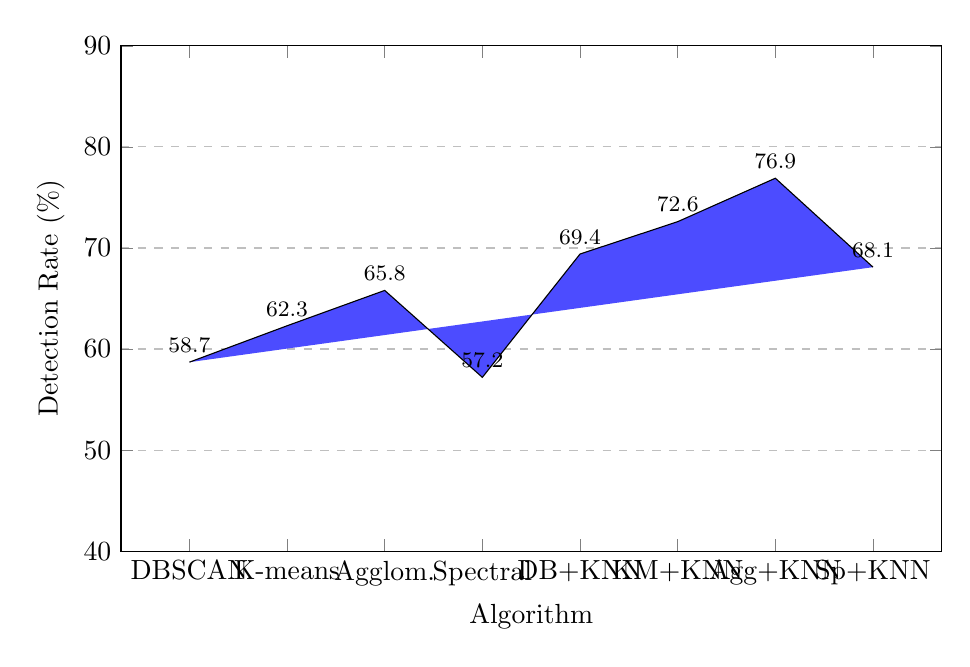
\begin{tikzpicture}
        \begin{axis}[
            width=12cm,
            height=8cm,
            ylabel={Detection Rate (\%)},
            xlabel={Algorithm},
            symbolic x coords={DBSCAN, K-means, Agglom., Spectral, DB+KNN, KM+KNN, Agg+KNN, Sp+KNN},
            xtick=data,
            ymin=40, ymax=90,
            ymajorgrids=true,
            grid style=dashed,
            nodes near coords,
            every node near coord/.append style={font=\footnotesize},
            ylabel near ticks,
            legend style={at={(0.5,1.05)}, anchor=south, legend columns=2},
            ]
            
            \addplot[fill=blue!70, draw=black] coordinates {
                (DBSCAN, 58.7)
                (K-means, 62.3)
                (Agglom., 65.8)
                (Spectral, 57.2)
                (DB+KNN, 69.4)
                (KM+KNN, 72.6)
                (Agg+KNN, 76.9)
                (Sp+KNN, 68.1)
            };
            
        \end{axis}
    \end{tikzpicture}
    \caption{Detection performance under extreme shadowing conditions}
    \label{fig:extreme_shadowing}
\end{figure}

\subsection{Computational Performance Comparison}

Table \ref{tab:computation_time} presents the average computation time required for each algorithm to process 100 time slots on the test hardware.

\begin{table}[htbp]
    \centering
    \caption{Average computation time for different algorithms (ms)}
    \label{tab:computation_time}
    \begin{tabular}{lcccc}
        \toprule
        \textbf{Algorithm} & \textbf{Scenario A} & \textbf{Scenario B} & \textbf{Scenario C} & \textbf{Average} \\
        \midrule
        DBSCAN & 65 & 64 & 66 & 65 \\
        K-means & 42 & 41 & 43 & 42 \\
        Agglomerative & 78 & 77 & 79 & 78 \\
        Spectral & 127 & 125 & 129 & 127 \\
        \midrule
        DBSCAN+KNN & 94 & 93 & 95 & 94 \\
        K-means+KNN & 67 & 66 & 68 & 67 \\
        Agglomerative+KNN & 112 & 111 & 113 & 112 \\
        Spectral+KNN & 162 & 160 & 164 & 162 \\
        \bottomrule
    \end{tabular}
\end{table}

\section{Symbol List}
\label{app:symbols}

Table \ref{tab:symbols} provides a comprehensive list of mathematical symbols used throughout this thesis.

\begin{table}[htbp]
    \centering
    \caption{List of mathematical symbols}
    \label{tab:symbols}
    \begin{tabular}{cl}
        \toprule
        \textbf{Symbol} & \textbf{Description} \\
        \midrule
        $\alpha$ & Path loss exponent \\
        $\sigma_{\psi}$ & Shadow fading standard deviation (dB) \\
        $d_{ij}$ & Distance between nodes $i$ and $j$ \\
        $P_t$ & Transmission power \\
        $P_r$ & Received power \\
        $\mu$ & Mean of RSS measurements \\
        $\sigma^2$ & Variance of RSS measurements \\
        $\gamma$ & Skewness of RSS distribution \\
        $\kappa$ & Kurtosis of RSS distribution \\
        $\epsilon$ & Distance threshold in DBSCAN \\
        $k$ & Number of neighbors in KNN \\
        $\delta$ & Refinement threshold for enhanced detection \\
        $C$ & Cluster assignments \\
        \bottomrule
    \end{tabular}
\end{table}


% Symbol List
\chapter*{Symbol List}
\addcontentsline{toc}{chapter}{Symbol List}
\begin{tabular}{cl}
$P_d$ & Probability of detection \\
$P_f$ & Probability of false alarm \\
$\gamma$ & Received signal power \\
$\sigma^2$ & Noise variance \\
$\lambda$ & Threshold value \\
$d_{ij}$ & Distance between data points $i$ and $j$ \\
$\epsilon$ & DBSCAN neighborhood radius \\
$k$ & Number of clusters in K-means \\
$\vect{x}$ & Feature vector \\
$\mat{D}$ & Distance matrix \\
\end{tabular}

\end{document}